% -*-latex-*-

\chapter{Spectrometer Optics Study}
\label{C6}

In \Cref{C5}, we have introduced the experimental setup of E08-027. The strong transverse target field and the septum field makes the reconstruction of the kinematics of the scattered electrons, i.e., the spectrometer optics study, to be a challenge.

In the usual optics study procedure, the HRS is considered as an identical pair of magnetic spectrometers, each of which contains three quadrupoles and a dipole magnet in a QQDQ configuration as mentioned in the previous chapter. An optics matrix is introduced to represent the effect of the magnets configuration. Using this optics matrix, the kinematic variables of the scattered particles at the interaction point can be reconstructed from the signals recorded in the detectors. The optics matrix elements are determined through an established optics calibration procedure. They have been optimized over the full momentum ranges of both spectrometers and have been tested and shown to be stable.

During E08-027, a pair of septum magnets were used to bend the electrons with scattering angles $\approx$ \SI{5.77}{\degree} into the minimum spectrometer angle \SI{12.5}{\degree} of the HRS. The optics study for HRS with septum was first performed during E97-110 \cite{Sulkosky2005}. In E97-110, the optics matrix was re-optimized with the septum magnet added into the QQDQ magnets configuration. The basic optimization procedure was almost the same as the normal optics calibration procedure of the HRS. This procedure is preserved in E08-027, and thus the optics matrix method is used to describe the joint effect of the septum magnet and the HRS magnets.

In addition to the septa magnets, the optics calibration procedure needs to be modified to accommodate the effect from the strong transverse magnetic field of the polarized NH${}_3$ target. For E08-027, this was done by separating the motion of the scattered electron into two parts: the motion in the target field region, which can be calculated using the equation of motion of charged particles in the magnetic field, and the motion out of the target field region, which is described by the optics matrix. The optics study procedure and the corresponding reconstruction procedure were adjusted following this idea. In this chapter, we will summarize the procedure of the spectrometer optics study for E08-027.

\section{Coordinate Systems}
\label{C6S1}

In this section, an overview of the target and focal plane coordinate systems used in the spectrometer optics study is presented. More details can be found in Ref. \cite{Liyanage2002}. All coordinate systems are Cartesian unless otherwise stated. Note that in this section all references to angular coordinates should be considered as referring to the tangent of the angle.

\subsection[Hall Coordinate System]{Hall Coordinate System (HCS)}
\label{C6S1SS1}

The origin of the HCS is at the center of the Hall A, which is defined to be the intersection point of the beam and the vertical axis of the target. The $\hat{z}$ axis is along the beam line and points downstream, the $\hat{y}$ axis is vertically up, and the $\hat{x}$ axis is horizontal and pointing to the left if looking along $\hat{z}$ and upright along $\hat{y}$, see \Cref{C6S1SS1F1}.

\begin{figure}[p!]
  \centering
  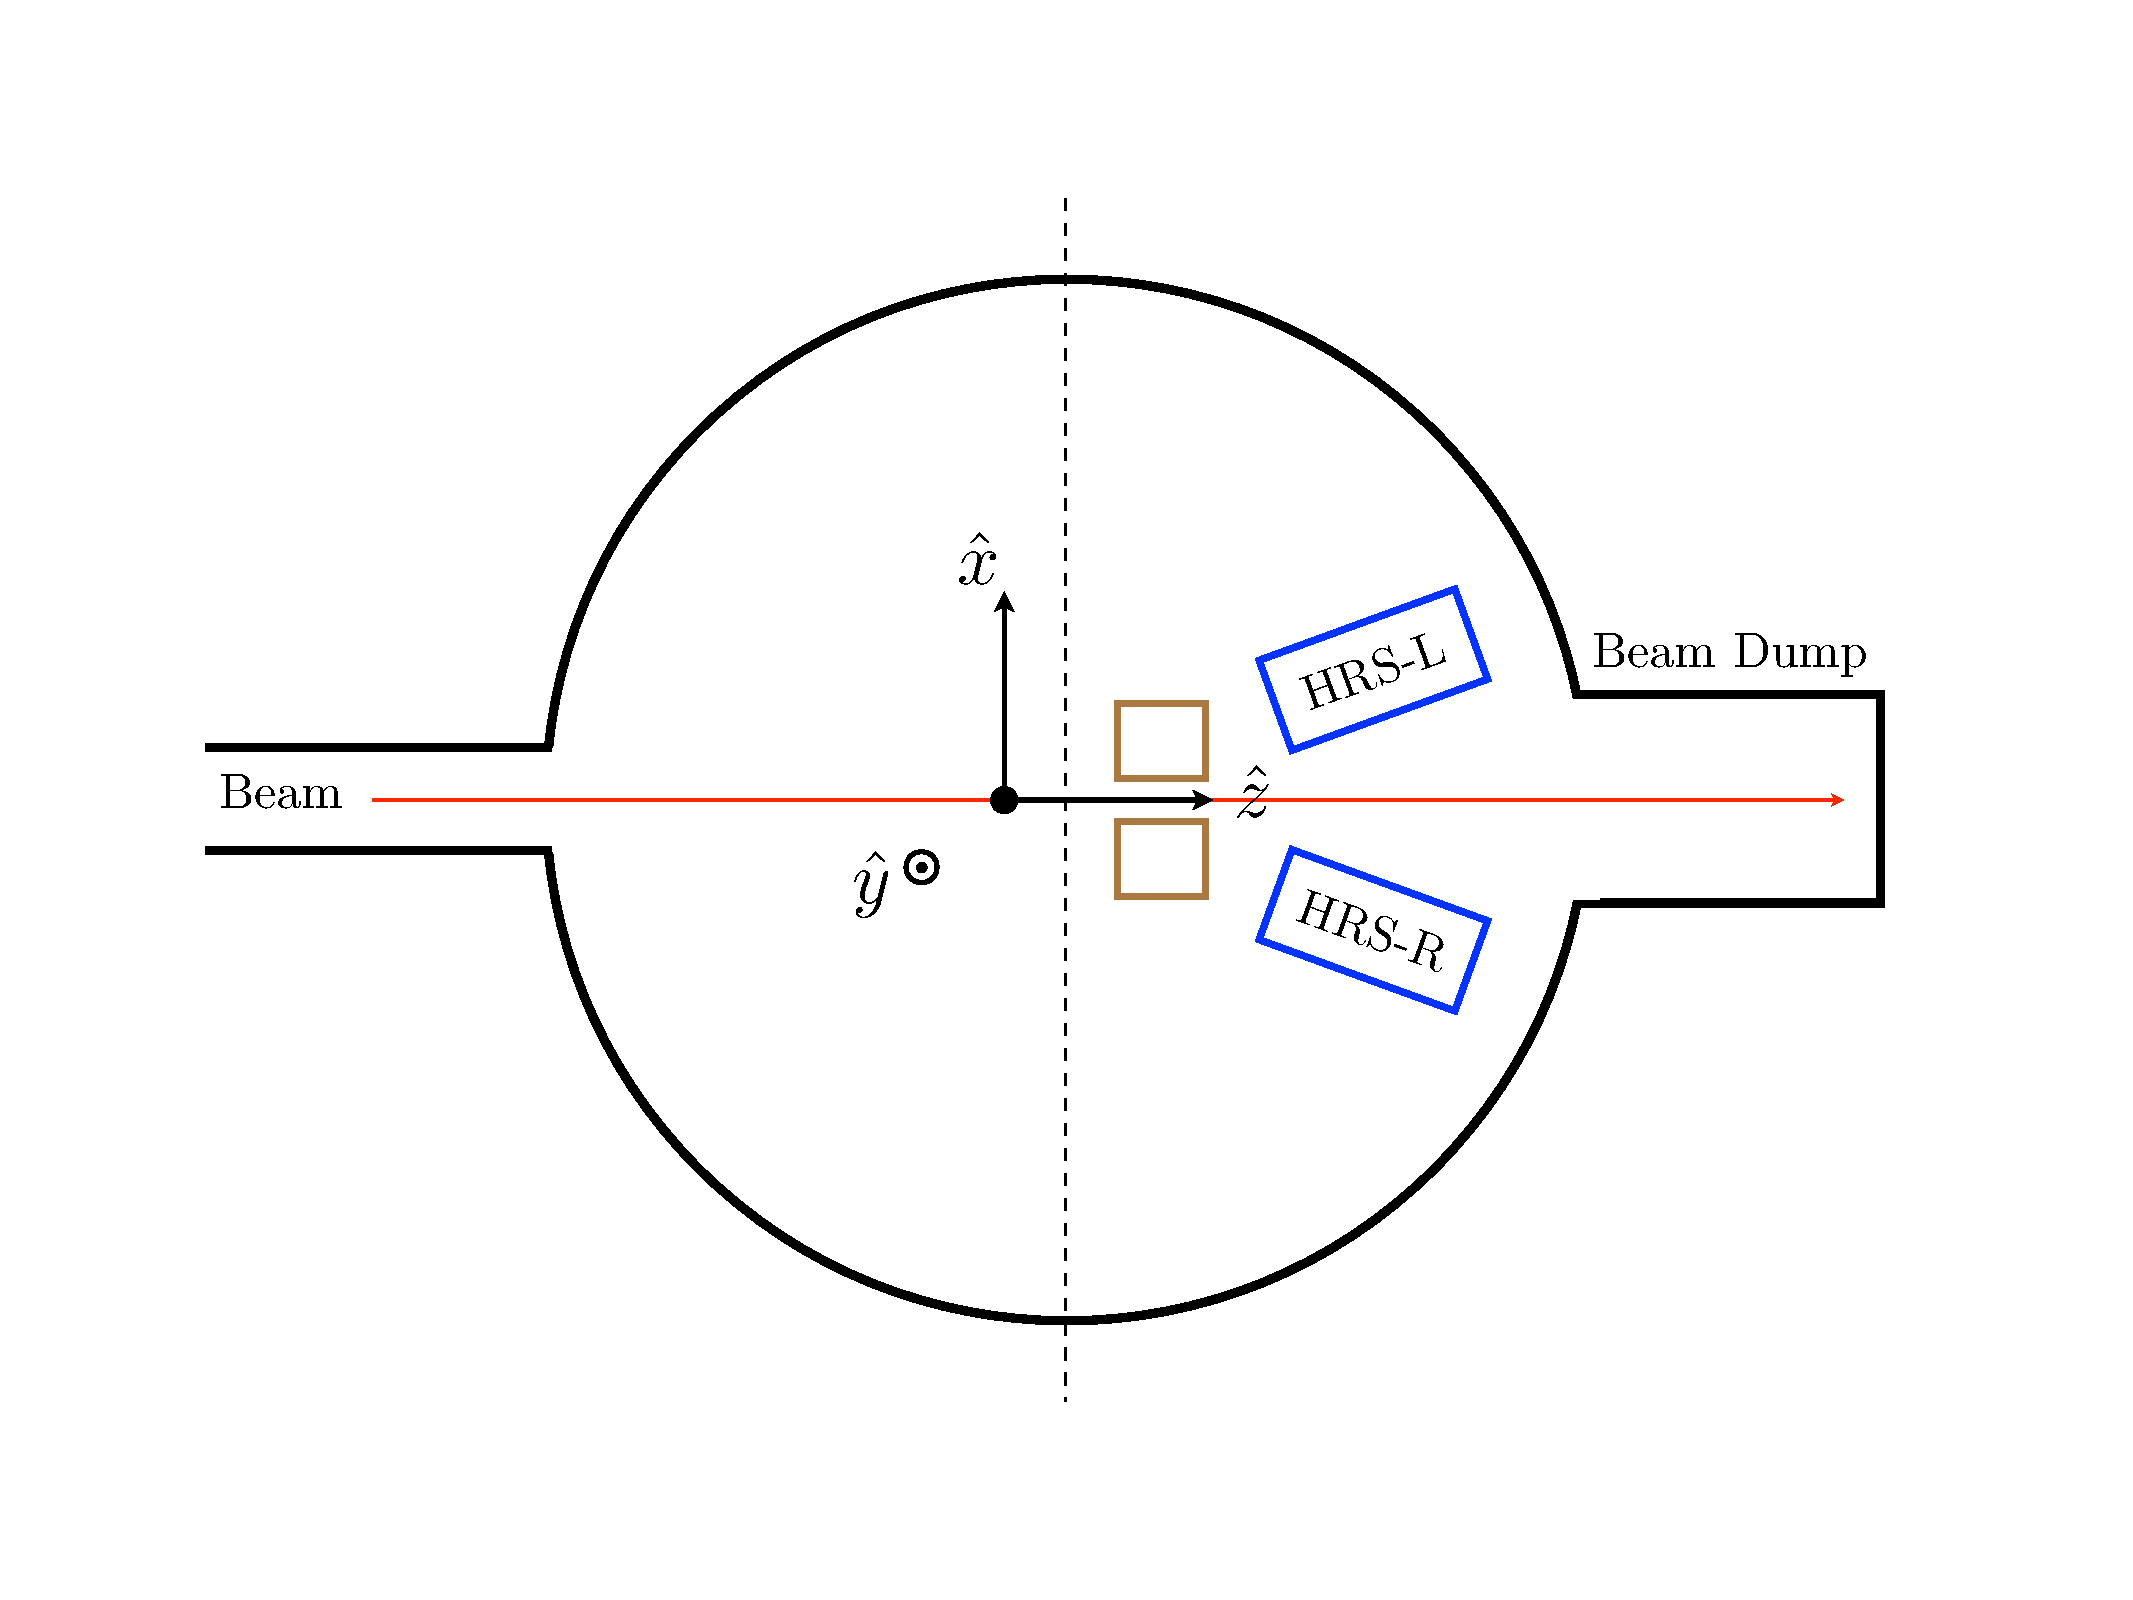
\includegraphics[width=0.75\textwidth]{figs/HCS.pdf}
  \caption[Hall coordinate system.]{Hall coordinate system (top view). \label{C6S1SS1F1}}
\end{figure}

\subsection[Target Coordinate System]{Target Coordinate System (TCS)}
\label{C6S1SS2}

\begin{figure}[p!]
  \centering
  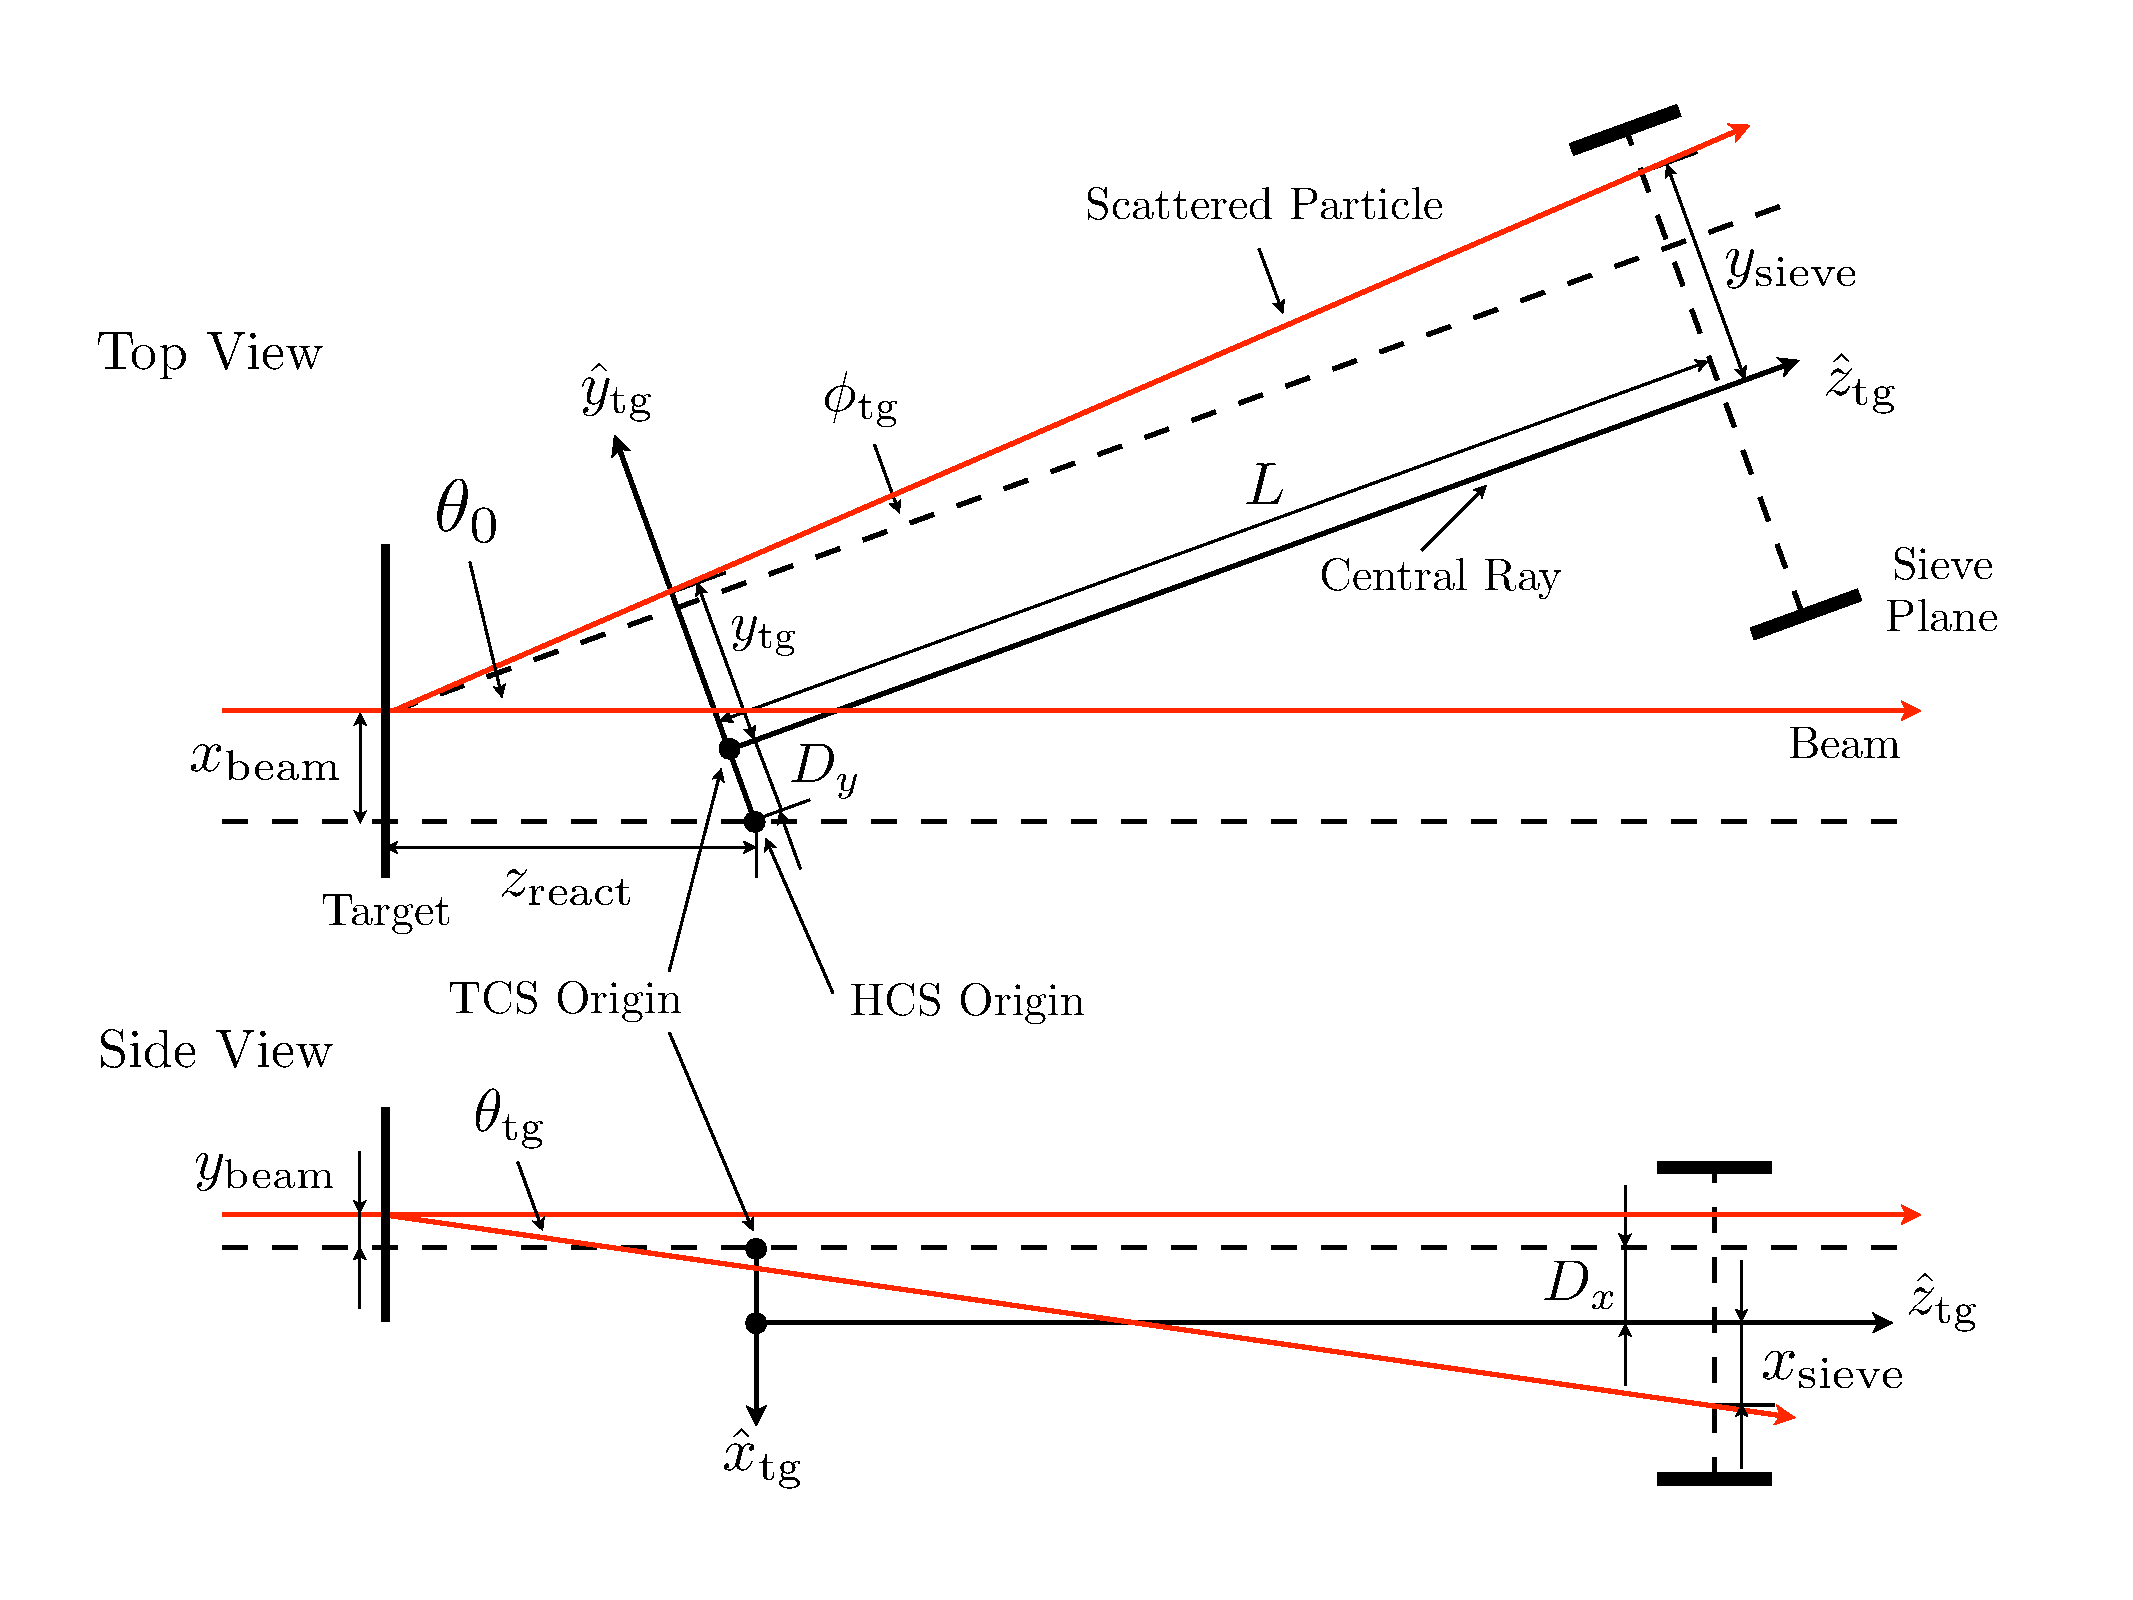
\includegraphics[width=0.9\textwidth]{figs/TCS.pdf}
  \caption[Target coordinate system.]{Target coordinate system (top and side views). $\theta_0$ is the spectrometer central angle, $L$ is the distance from the sieve slit to the TCS origin, $D_x$ and $D_y$ are the vertical and horizontal deviations of the spectrometer central ray to the HCS origin. \label{C6S1SS2F1}}
\end{figure}

Each of the two spectrometers has its own TCS. The $\hat{z}_{\mathrm{tg}}$ axis of the TCS is defined by the central ray of the sieve collimator for a given spectrometer which is the line perpendicular to the plane of the sieve slit passing through the center point of the central sieve slit hole. The $\hat{z}_{\mathrm{tg}}$ points away from the target towards the spectrometer and $\hat{x}_{\mathrm{tg}}$ is vertically down. Thus $\hat{y}_{\mathrm{tg}}$ is pointing to the left if looking along the $\hat{z}_{\mathrm{tg}}$ direction. Ideally, the $\hat{z}_{\mathrm{tg}}$ axis should pass through the hall center if the spectrometer points directly to the hall center and the sieve slit is perfectly centered. In this ideal case, the origin of the TCS coincides with the origin of the HCS. However, the origin of the TCS typically deviates from the hall center. The deviation can be measured by surveying the spectrometer pointing. The angle between $\hat{z}_{\mathrm{tg}}$ of the TCS and the $\hat{z}$ of the HCS is defined as the central angle $\theta_0$ of the spectrometer.

The kinematics of each scattering event is expressed as four variables in the TCS: the out-of-plane angle $\optt{tg}$ and the in-plane $\optp{tg}$ angle with respect to the central ray are given by $\mathrm{d}x/\mathrm{d}z$ and $\mathrm{d}y/\mathrm{d}z$ in the TCS; $\opty{tg}$ is given by the $y$ coordinate of the intersection point of the scattered particles's trajectory and the $z_{\mathrm{tg}}=0$ plane. The fourth variable $\delta$ is related to the momentum of the scattered particle:
\begin{equation} \label{C6S1SS2E1}
\delta = \frac{P-P_0}{P_0},
\end{equation}
where $P$ is the measured momentum of a particle and $P_0$ is the central momentum setting of HRS and septum \cite{Liyanage2002}. The scattering angle of the scattered particle can be calculated from the TCS variables:
\begin{equation} \label{C6S1SS2E2}
\optt{scat} = \arccos\left(\frac{\cos(\theta_0)-\optp{tg}\sin(\theta_0)}{\sqrt{1+\theta_{\mathrm{tg}}^2+\phi_{\mathrm{tg}}^2}}\right),
\end{equation}
where $\theta_0$ is the spectrometer certral angle. A diagram of the TCS as well as its relations with the HCS for the left arm is shown in \Cref{C6S1SS2F1}.

\subsection[Detector Coordinate System]{Detector Coordinate System (DCS)}
\label{C6S1SS3}

\begin{figure}[tb!]
  \centering
  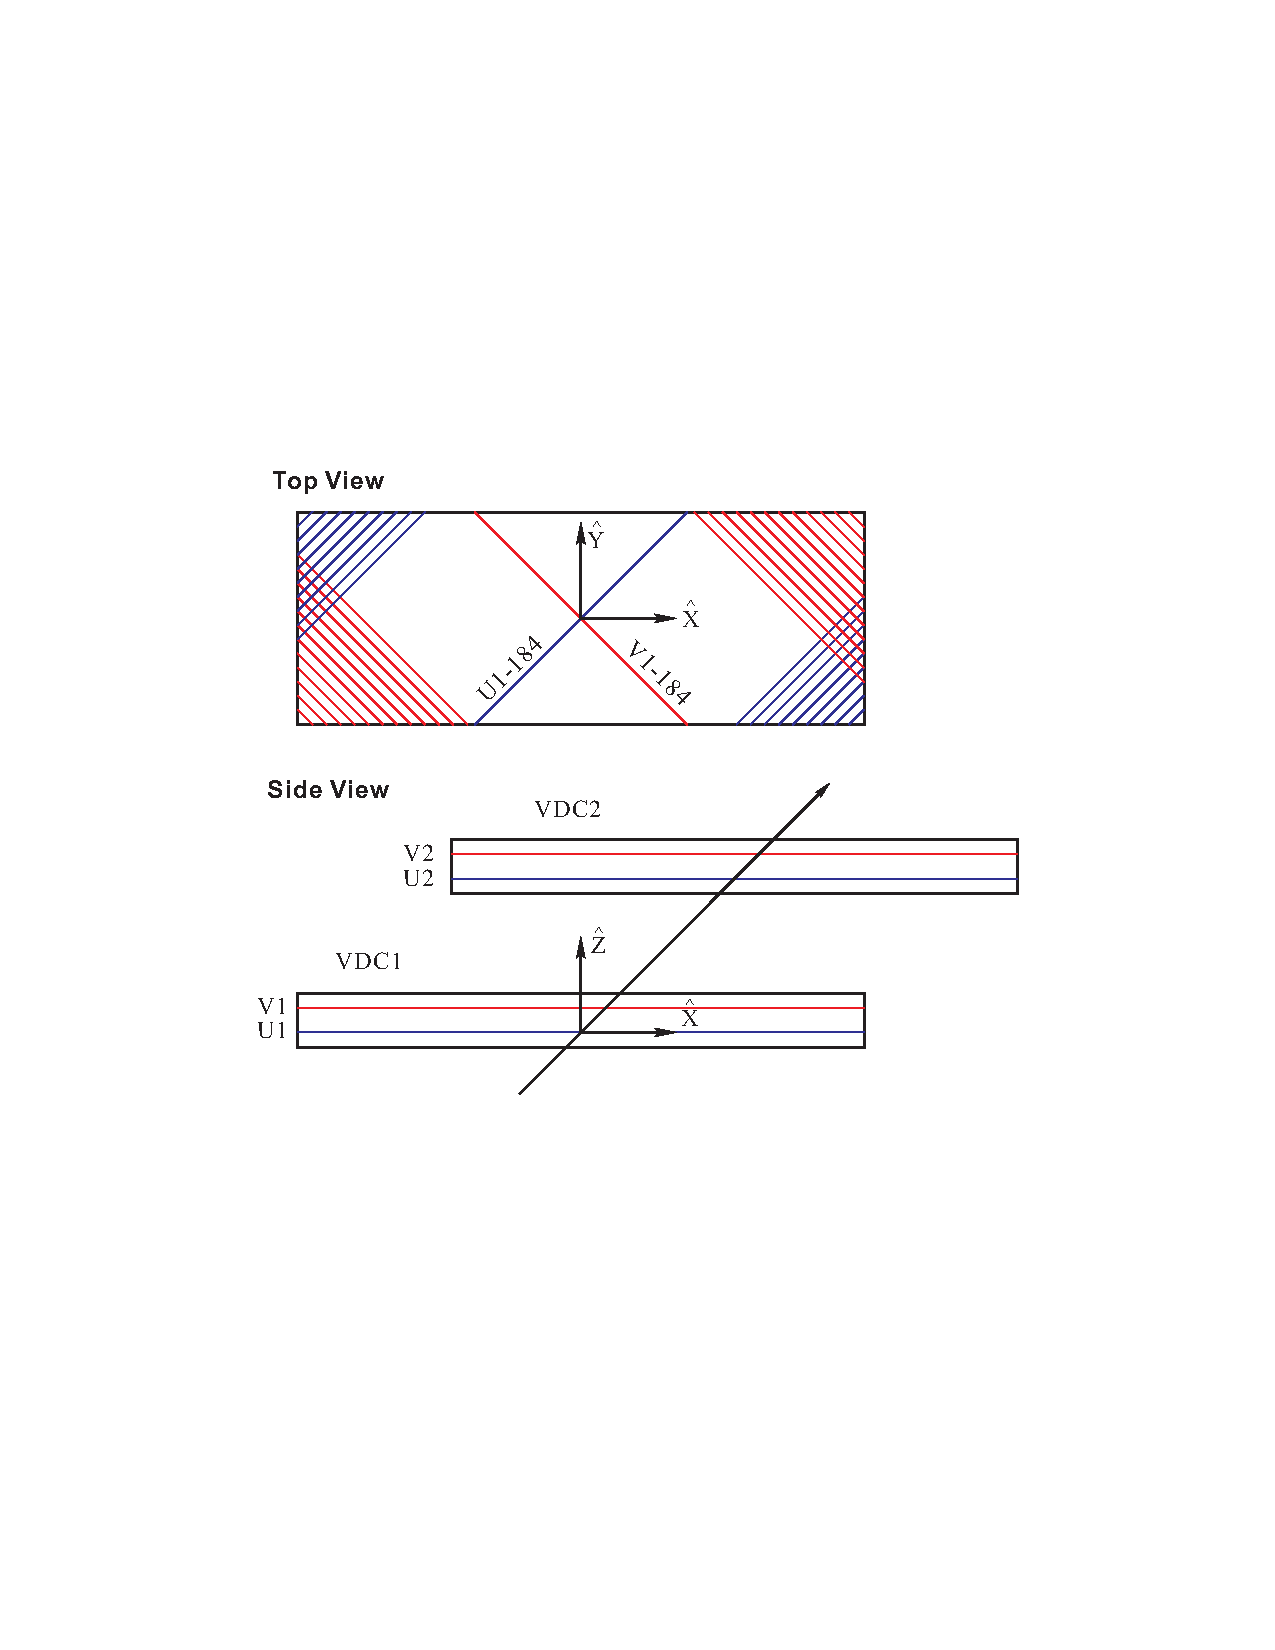
\includegraphics[width=0.75\textwidth]{figs/DCS.pdf}
  \caption[Detector coordinate system.]{Detector coordinate system (top and side views). The intersection point of the wire 184 of the U1 plane and the perpendicular projection of wire 184 of the V1 plane onto the U1 plane is shown in the top view. Plot reproduced from \cite{Qiang2007}. \label{C6S1SS3F1}}
\end{figure}

The coordinates of the detected particles are measured by the VDCs, as described in \Cref{C5}. The origin of the DCS is given by the intersection point of wire 184 of the VDC1 U1 plane and the perpendicular projection of wire 184 in the VDC1 V1 plane onto the VDC1 U1 plane. $\hat{z}_{\mathrm{det}}$ is perpendicular to the VDC plane pointing vertically up, and the $\hat{x}_{\mathrm{det}}$ is parallel to the long symmetry axis of the lower VDC pointing downstream. Thus the $\hat{y}_{\mathrm{det}}$ is parallel to the short symmetry axis of the lower VDC. See \Cref{C6S1SS3F1}. When a particle is detected, two spatial coordinates $\optx{det}$, $\opty{det}$ and two angular coordinates $\optt{det}\equiv\mathrm{d}x_{\mathrm{det}}/\mathrm{d}z_{\mathrm{det}}$, $\optp{det}\equiv\mathrm{d}y_{\mathrm{det}}/\mathrm{d}z_{\mathrm{det}}$ are calculated in this coordinate system.

\subsection[Transport Coordinate System at the Focal Plane]{Transport Coordinate System (TRCS) at the Focal Plane}
\label{C6S1SS4}

The TRCS at the focal plane is given by rotating the DCS around the $y$ axis by \SI{45}{\degree} clockwise if viewing along $y$ axis. Ideally, the $\hat{z}_{\mathrm{tra}}$ coincides with the central ray of the spectrometer. Typically, it is used to transport the DCS to the focal plane coordinate system. The TRCS coordinates of an event can be calculated from the DCS coordinates by:
\begin{align} \label{C6S1SS4E1}
\optx{tra} & = \optx{det}\cos(\rho_0)(1+\optt{tra}\tan(\rho_0)), \displaybreak[0] \\ \label{C6S1SS4E2}
\optt{tra} & = \frac{\optt{det}+\tan(\rho_0)}{1-\optt{det}\tan(\rho_0)}, \\  \label{C6S1SS4E3}
\opty{tra} & = \opty{det}+\sin(\rho_0)\optp{tra}\optx{det}, \\ \label{C6S1SS4E4}
\optp{tra} & = \frac{\optp{det}}{\cos(\rho_0)(1-\optt{det}\tan(\rho_0))},
\end{align}
where $\rho_0=-$\SI{45}{\degree}.

\subsection[Focal Plane Coordinate System]{Focal Plane Coordinate System (FCS)}
\label{C6S1SS5}

\begin{figure}[b!]
  \centering
  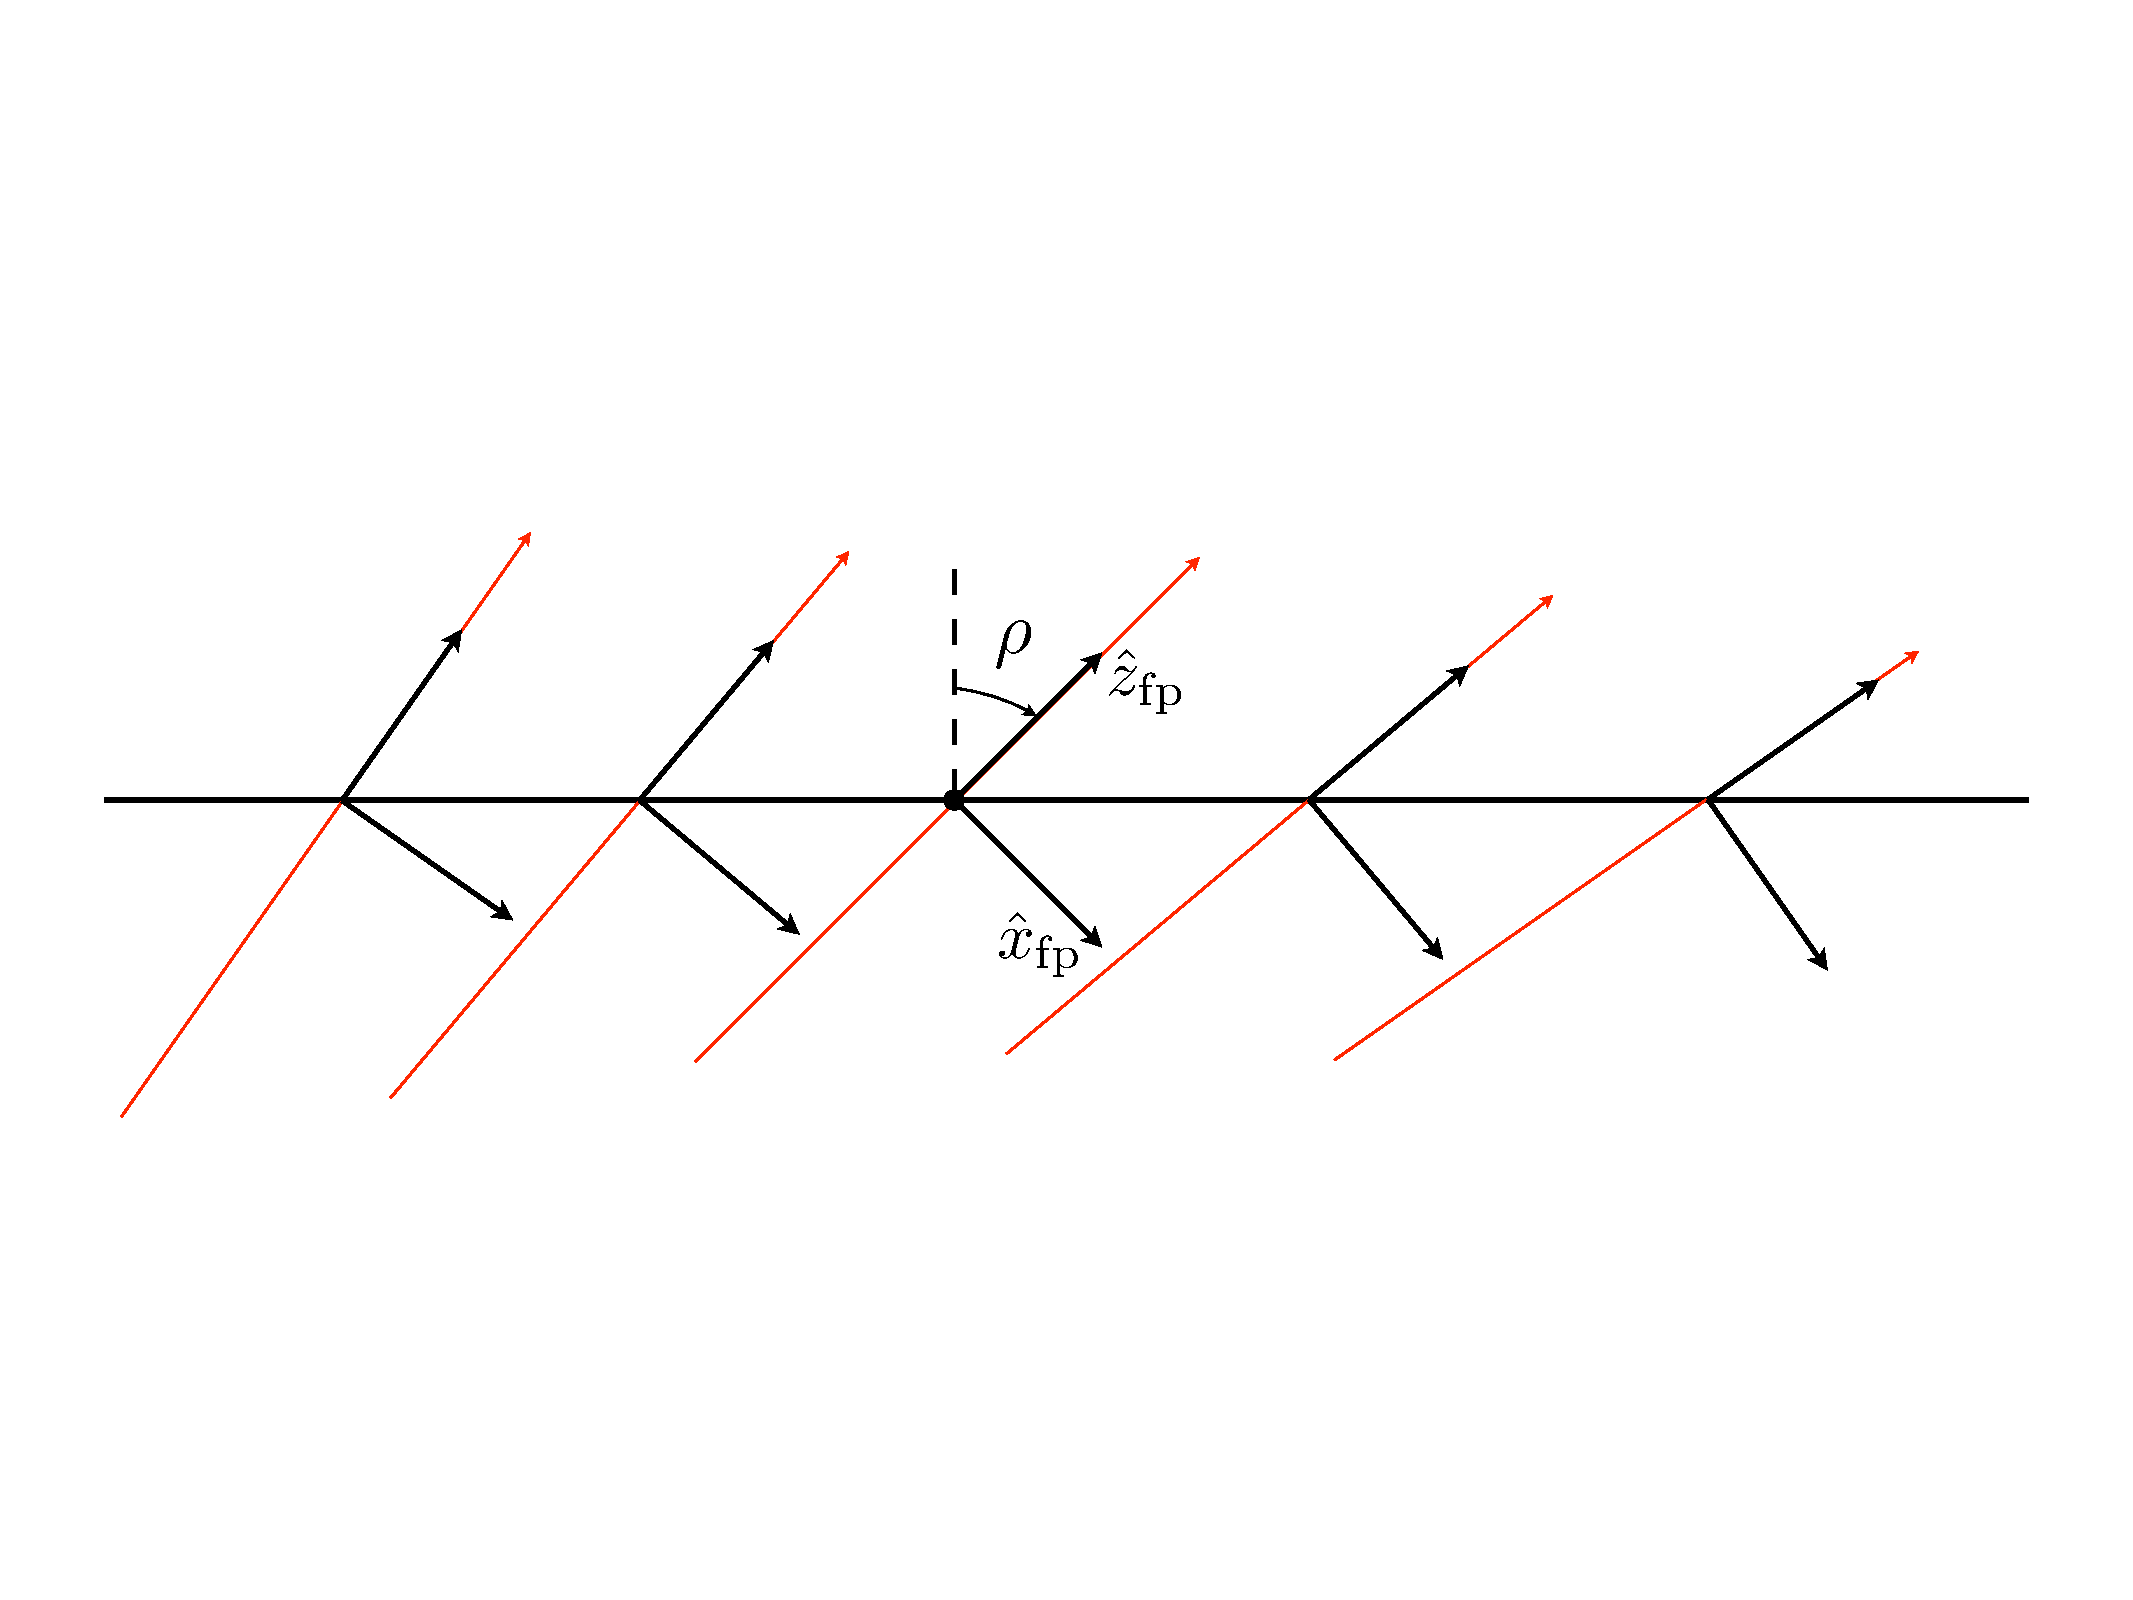
\includegraphics[width=0.7\textwidth]{figs/FCS.pdf}
  \caption[Focal plane coordinate system.]{Focal plane coordinate system. The red trajectories are the local certral rays with $\optt{tg}=\optp{tg}=0$. \label{C6S1SS5F1}}
\end{figure}

The FCS is a rotated coordinate system with its $z$ axis always parallel to the local central ray, which is defined as the trajectory of a particular particle with $\optt{tg}=\optp{tg}=0$ in the TCS for each relative momentum. This coordinate system is generated by rotating the DCS clockwise around its $y$ axis by the angle $\rho$ between the local central ray and the $z$ axis of the DCS. See \Cref{C6S1SS5F1}. Because of the focusing of the HRS magnet system, particles with the same scattering momentum will be focused at the focal plane, which means the relative momentum to the central momentum of the spectrometer is approximately a function of $\optx{tra}$. Therefore, the rotating angle $\rho$ is a function of $\optx{tra}$. As a result, the dispersive angle $\optt{fp}$ is small for all points across the focal plane in this rotated coordinate system, thus the expansion of the optics matrix will converge faster during the calibration, which will greatly simplify the optimizing procedure. The FCS coordinates of an event can be calculated form the DCS and TRCS coordinates by:
\begin{align} \label{C6S1SS5E1}
\optx{fp} & = \optx{tra} \\ \label{C6S1SS5E2}
\optt{fp} & = \frac{\optt{det}+\tan(\rho)}{1-\optt{det}\tan(\rho)} \\ \label{C6S1SS5E3}
\opty{fp} & = \opty{tra}-\sum_i C_{i000}^{\,y} \optx{fp}^i \\ \label{C6S1SS5E4}
\optp{fp} & = \frac{\optp{det}-\sum_i C_{i000}^{\,p}\optx{fp}^i}{\cos(\rho)(1-\optt{det}\tan(\rho))},
\end{align}
where $\tan(\rho) = \sum C_{i000}^{\,t} \optx{fp}^i$. The coefficients $C_{i000}^{\,t}$, $C_{i000}^{\,y}$ and $C_{i000}^{\,p}$ also include corrections for the systematic offsets due to misalignment of VDC packages.

\section{Optimization Procedure}
\label{C6S2}

\subsection{Optics Matrix}
\label{C6S2SS1}

As mentioned above, the DCS coordinates $\optx{det}$, $\optt{det}$, $\opty{det}$, $\optp{det}$ are directly measured with the VDC package. The optics matrix method allows a unique one-to-one mapping between these variables and the TCS variables, $\optx{tg}$, $\optt{tg}$, $\opty{tg}$, $\optp{tg}$ and $\delta$.

 During the optics calibration, the $\optx{tg}$ is effectively set at zero, therefore the unknowns at the target are reduced to four: $\delta$, $\optt{tg}$, $\opty{tg}$, $\optp{tg}$. Thus, the optics matrix can be expressed as (in a first-order approximation):
\begin{equation} \label{C6S2SS1E1}
\left(
\begin{matrix} \delta \\ \theta \\ y \\ \phi \end{matrix}
\right)_{\mathrm{tg}} = \left(
\begin{matrix}
\left<\delta|x\right> & \left<\delta|\theta\right> & 0 & 0 \\
\left<\theta|x\right> & \left<\theta|\theta\right> & 0 & 0 \\
0 & 0 & \left<y|y\right> & \left<y|\phi\right> \\
0 & 0 & \left<\phi|y\right> & \left<\phi|\phi\right>
\end{matrix}
\right)
\left(\begin{matrix} x \\ \theta \\ y \\ \phi \end{matrix}
\right)_{\mathrm{fp}}.
\end{equation}

In practice, the matrix takes a more complicated form: a set of tensors $D_{jkl}$, $T_{jkl}$, $Y_{jkl}$ and $P_{jkl}$, which are polynomials of $\optx{fp}$, links the FCS coordinates to TCS coordinates for each target variables. For example:
\begin{gather} \label{C6S2SS1E2}
\optt{tg} = \sum_{j,k,l} T_{jkl} \optt{fp}^j \opty{fp}^k \optp{fp}^l, \\ \label{C6S2SS1E3}
T_{jkl} = \sum_i C_{ijkl}^{T} \optx{fp}^i,
\end{gather}
where $C_{ijkl}^{T}$ are the optics matrix elements for $\optt{tg}$. Similar expressions can be written for $\delta$, $\opty{tg}$ and $\optp{tg}$. The summation over $i$, $j$, $k$ and $l$ is carried out and optimized up to the third order. The main purpose of the optimization procedure is to determine all optics matrix elements using dedicated optics calibration data, described in the next section.

\subsection{Matrix Optimization without Target Field}
\label{C6S2SS2}

The optics optimization procedure is always performed on a set of data with wide coverage on the entire acceptance of the spectrometer, which includes $\delta$ for momentum, $\optt{tg}$ and $\optp{tg}$ for solid angle and $\opty{tg}$ for reaction position. The target variables $\delta$, $\optt{tg}$, $\opty{tg}$ and $\optp{tg}$ for the calibration data set has to be precisely known. This requirement can be fulfilled by using survey results combined with a sieve-slit collimator for $\optt{tg}$ and $\optp{tg}$ and a foil target for $\opty{tg}$ and some well-known physics process like elastic scattering for $\delta$ as explained in this section.

\begin{figure}[tb!]
  \centering
  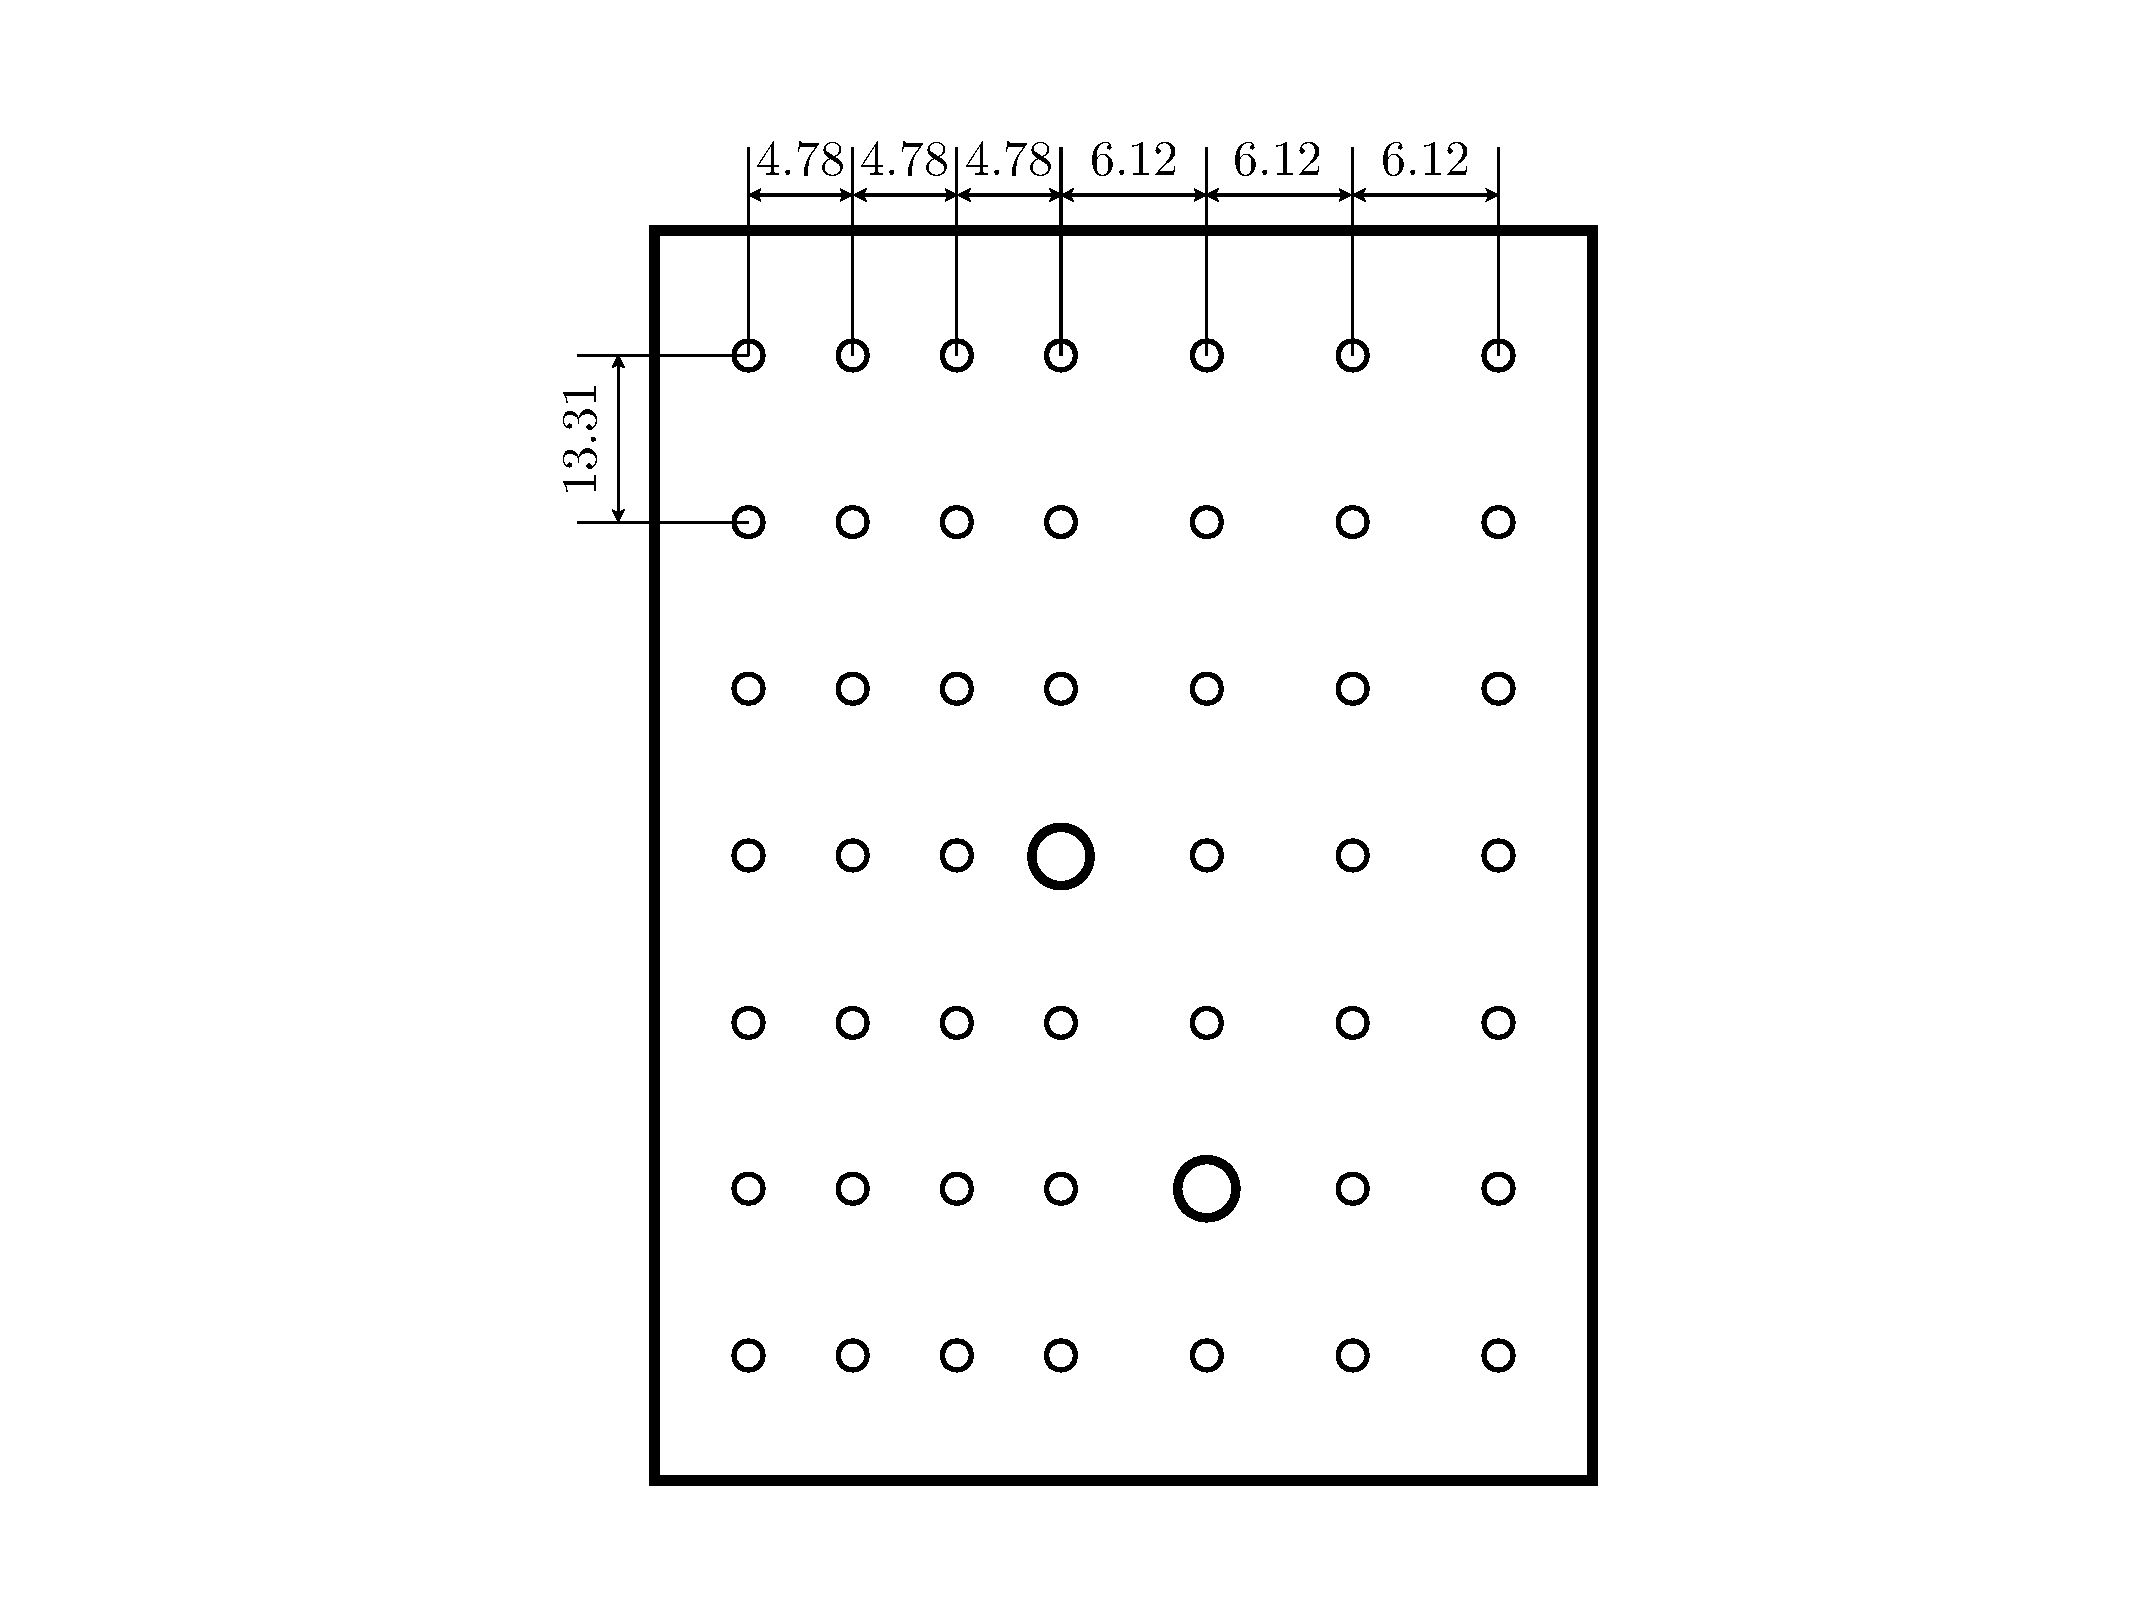
\includegraphics[width=0.3\textwidth]{figs/sieve-slit.pdf}
  \caption[Geometric configuration of the sieve slit.]{Geometric configuration of the sieve slit used during E08-027. The dimensions are in mm. The two large holes are used to determine the orientation of the sieve slit. The diameters are 1.4 mm and 2.7 mm for the normal holes and the large holes, respectively. \label{C6S2SS2F1}}
\end{figure}

To calibrate $\optt{tg}$, $\optp{tg}$ and $\opty{tg}$, a fixed energy electron beam with a point-like profile is incident on a set of foil target. The target foils are aligned along the beam line to cover the $\opty{tg}$ acceptance. Therefore, the HCS coordinates $\optx{beam}$ and $\opty{beam}$ of the interaction point can be determined by BPM, and the $z$ coordinate $\optz{react}$ can be determined by the survey result of the target foil. On the other side, a sieve slit collimator is placed before the entrance of the spectrometer (if there is a septum magnet, it is placed before the entrance of the septum magnet). A figure of the sieve slit used in E08-027 is shown in \Cref{C6S2SS2F1}. The sieve has holes that are arranged in a grid pattern with well-defined horizontal and vertical coordinates $\optx{sieve}$ and $\opty{sieve}$ (in TCS) covering the angular acceptance. The in-plane angle $\optp{tg}$ and the out-of-plane angle $\optt{tg}$ for each hole can be expressed as:
\begin{align} \label{C6S2SS2E1}
\optt{tg} & = \frac{\optx{sieve}+D_x+\opty{beam}}{L-\optz{react}\cos(\theta_0)-\optx{beam}\sin(\theta_0)}, \\ \label{C6S2SS2E2}
\optp{tg} & = \frac{\opty{sieve}+D_y-\optx{beam}\cos(\theta_0)+\optz{react}\sin(\theta_0)}{L-\optz{react}\cos(\theta_0)-\optx{beam}\sin(\theta_0)},
\end{align}
where $\theta_0$ is the spectrometer central angle, $L$ is the distance from the sieve slit to the TCS origin and the $D_x$ and $D_y$ are the vertical and horizontal deviations of the spectrometer central ray from the HCS origin, respectively, see \Cref{C6S1SS2F1}. $L$, $D_x$ and $D_y$ can be determined by surveying the spectrometer. The spectrometer central angle $\theta_0$ can be calculated from the geometries of the sieve slit and the target or by performing a pointing measurement using the energy deviation between the elastic peaks of two different nuclei \cite{Liyanage2011}. Precise determination of $\optt{tg}$ and $\optp{tg}$ is important because they determine the scattering angle via \cref{C6S1SS2E2}. With $\optt{tg}$ and $\optp{tg}$ known from \cref{C6S2SS2E1,C6S2SS2E2}, the spatial coordinates $\optx{tg}$ and $\opty{tg}$ can be expressed as:
\begin{align} \label{C6S2SS2E3}
\optx{tg} & = \optx{sieve}-L\optt{tg}, \\ \label{C6S2SS2E4}
\opty{tg} & = \opty{sieve}-L\optp{tg}.
\end{align}

To calibrate $\delta$, some well-known physics process can be used to determine the momentum of the detected particle. Take elastic scattering as example, the scattering momentum can be expressed as:
\begin{equation} \label{C6S2SS2E5}
P(M,\theta) = E' = \frac{E}{1+E/M(1-\cos(\theta))},
\end{equation}
where $E$ is the beam energy, $M$ is the target mass and $\theta$ is the scattering angle. Therefore, the target variable $\delta$ can be obtained from the calculated $P$ and the spectrometer central momentum $P_0$ by \cref{C6S1SS2E1}. To cover the acceptance range of $\delta$ of the HRS, several different $P_0$ values are used during the data collection to perform a so-called ``delta scan''. The energy loss of the scattered electrons due to the radiative effect when the electrons pass through the target material is considered as a correction to $\delta$.

As described above, the target variables $\optt{tg}$, $\opty{tg}$, $\optp{tg}$ and $\delta$ calculated from survey results (\cref{C6S2SS2E1,C6S2SS2E2,C6S2SS2E3,C6S2SS2E4}) or elastic scattering conditions (\cref{C6S2SS2E5}) are assumed to be the true value of the events in the data set collected with the sieve slit or elastic scattering. The optics matrix elements are then obtained by the minimizing of the aberration functions:
\begin{equation} \label{C6S2SS2E6}
\Delta (W) = \sum_s\left[\frac{\sum_{ijkl}C_{ijkl}^{W}\optx{fp}^i\optt{fp}^j\opty{fp}^k\optp{fp}^l-W^{0}}{\sigma_W^s}\right]^2,
\end{equation}
where $s$ is the total number of the events measured for optics calibration, $W$ can be any target variables $\delta$, $\optt{tg}$, $\opty{tg}$ or $\optp{tg}$ and $W_0$ is the corresponding reference variable calculated from survey results and the elastic condition. A C++ package based on the Hall A Analyzer \cite{Hansen2015} is developed to do this optimization, which is adopted from N. Liyanage's original code \cite{Liyanage2002} for ESPACE \cite{ESPACE}. The core of this package is the MIGRAD algorithm in the TMinuit package of ROOT \cite{ROOT}. The magnetic field simulation package SNAKE is used to generate an initial optics matrix for the optimization. This initial optics matrix accounts for the effects of the HRS magnets and the septum magnet. The package also contains a script for users to select events for optimization and some test scripts to compare the survey calculations with the reconstructed target variables.

\subsection{Target Field Effect}
\label{C6S2SS3}

As mentioned in \Cref{C5S3}, the field used to polarize the NH${}_3$ target is provided by a superconducting magnet, formed by a pair of Helmholtz coils. The field map of these coils has been directly calculated using the Biot-Savart law using the current density distribution of these coils. To estimate the uncertainty of this calculation, a measurement of the target field was performed during the experiment. The results indicate that the relative uncertainty of this field map is less than 1.2\% over the whole field region. The details of the field map are discussed in \Cref{A2}. The field map is calculated under the 5.0 T case and is scaled by 0.5 for the 2.5 T configuration.

The most important step during the optimization procedure in \Cref{C6S2SS2} is to determine the target plane variables for events collected during calibration runs. If there is no target field, the calculation of these variables only involves the linear projection between the sieve and the target and is straight forward. However, the linear projection is broken by the target field since the trajectory of the scattered electron is now a curve in the presence of this field.

A simulation package was developed to study the behavior of the scattered electrons in the target field. In order to do this, the equation of motion of the scattered electrons is integrated in the target field. The package uses the Runge-Kutta-Nystrom (RKN) method to do the integration. The trajectory of the electrons is approximated by chords in the integration method. For each chord, the deviation between its middle point and the real curve is also estimated by RKN method. The step size of the integration is adjusted dynamically to limit the integration uncertainty to $\leq$0.5 mm.

The trajectory of the scattered electron is also affected by the radiation effects when target field exists. The momentum of the electron decreases during the motion due to the energy loss. If there is no target field, the linear projection would not be influenced by the decreased momentum, but the curved trajectory of the scattered electron in the presence of the target field might change. This effect is also calculated in the simulation package. More details of the radiation effects can be found in reference \cite{Liu2015}.

With the help of the simulation package, the motion of the scattered electron in the target field region can be isolated. Since the field strength drops to less than 10 Gauss by the middle of the sieve slit, the sieve slit is taken as the edge of the target field region. Thus, the motion is separated into two parts: the first segment is from the interaction point to the sieve slit, where the trajectory can be calculated from the equation of motion, and the second segment is from the sieve slit to the focal plane, which can be described by the optics matrix.

\subsection{Matrix Optimization Revised}
\label{C6S2SS4}

The original optimization procedure had to be modified due to the presence of the target field. The reference values $W_0$ in \cref{C6S2SS2E6} can not be directly calculated from the survey results in this case. The new reference values are determined using the simulation package. The procedure to calculate new reference values involves the following steps:
\begin{enumerate}[parsep=0pt]
\item Select an elastic event, determine the coordinates of its interaction point ($\optx{react}$, $\opty{react}$, $\optz{react}$) and the coordinates of the sieve hole which it passes through ($\optx{sieve}$, $\opty{sieve}$);
\item Randomly generate a pair of scattering angles in TCS ($\optt{test}$, $\optp{test}$) and use \cref{C6S1SS2E2,C6S2SS2E5} to calculate the momentum $P_{\mathrm{elastic}}$ of the elastically scattered electron with this scattering angle;
\item \label{C6S2SS4A1} Set ($\optx{beam}$, $\opty{beam}$, $\optz{react}$) as start point and set $P_{\mathrm{elastic}}$ and ($\optt{test}$, $\optp{test}$) as the magnitude and direction of the momentum respectively, use the simulation package to generate a trajectory from the start point to sieve slit, assuming the coordinates of the intersection point of this trajectory and the sieve slit are ($\optx{drift}$, $\opty{drift}$);
\item \label{C6S2SS4A2} Compare ($\optx{drift}$, $\opty{drift}$) with ($\optx{sieve}$, $\opty{sieve}$), calculate the new test scattering angle:
\begin{align} \label{C6S2SS4E1}
\optt{test}^{\,\mathrm{new}} & = \optt{test}^{\,\mathrm{old}}+\frac{(\optx{drift}-\optx{sieve})/L}{2}, \\ \label{C6S2SS4E2}
\optp{test}^{\,\mathrm{new}} & = \optp{test}^{\,\mathrm{old}}+\frac{(\opty{drift}-\opty{sieve})/L}{2},
\end{align}
where $L$ is the distance from the sieve slit to the TCS origin;

\begin{figure}[tb!]
  \centering
  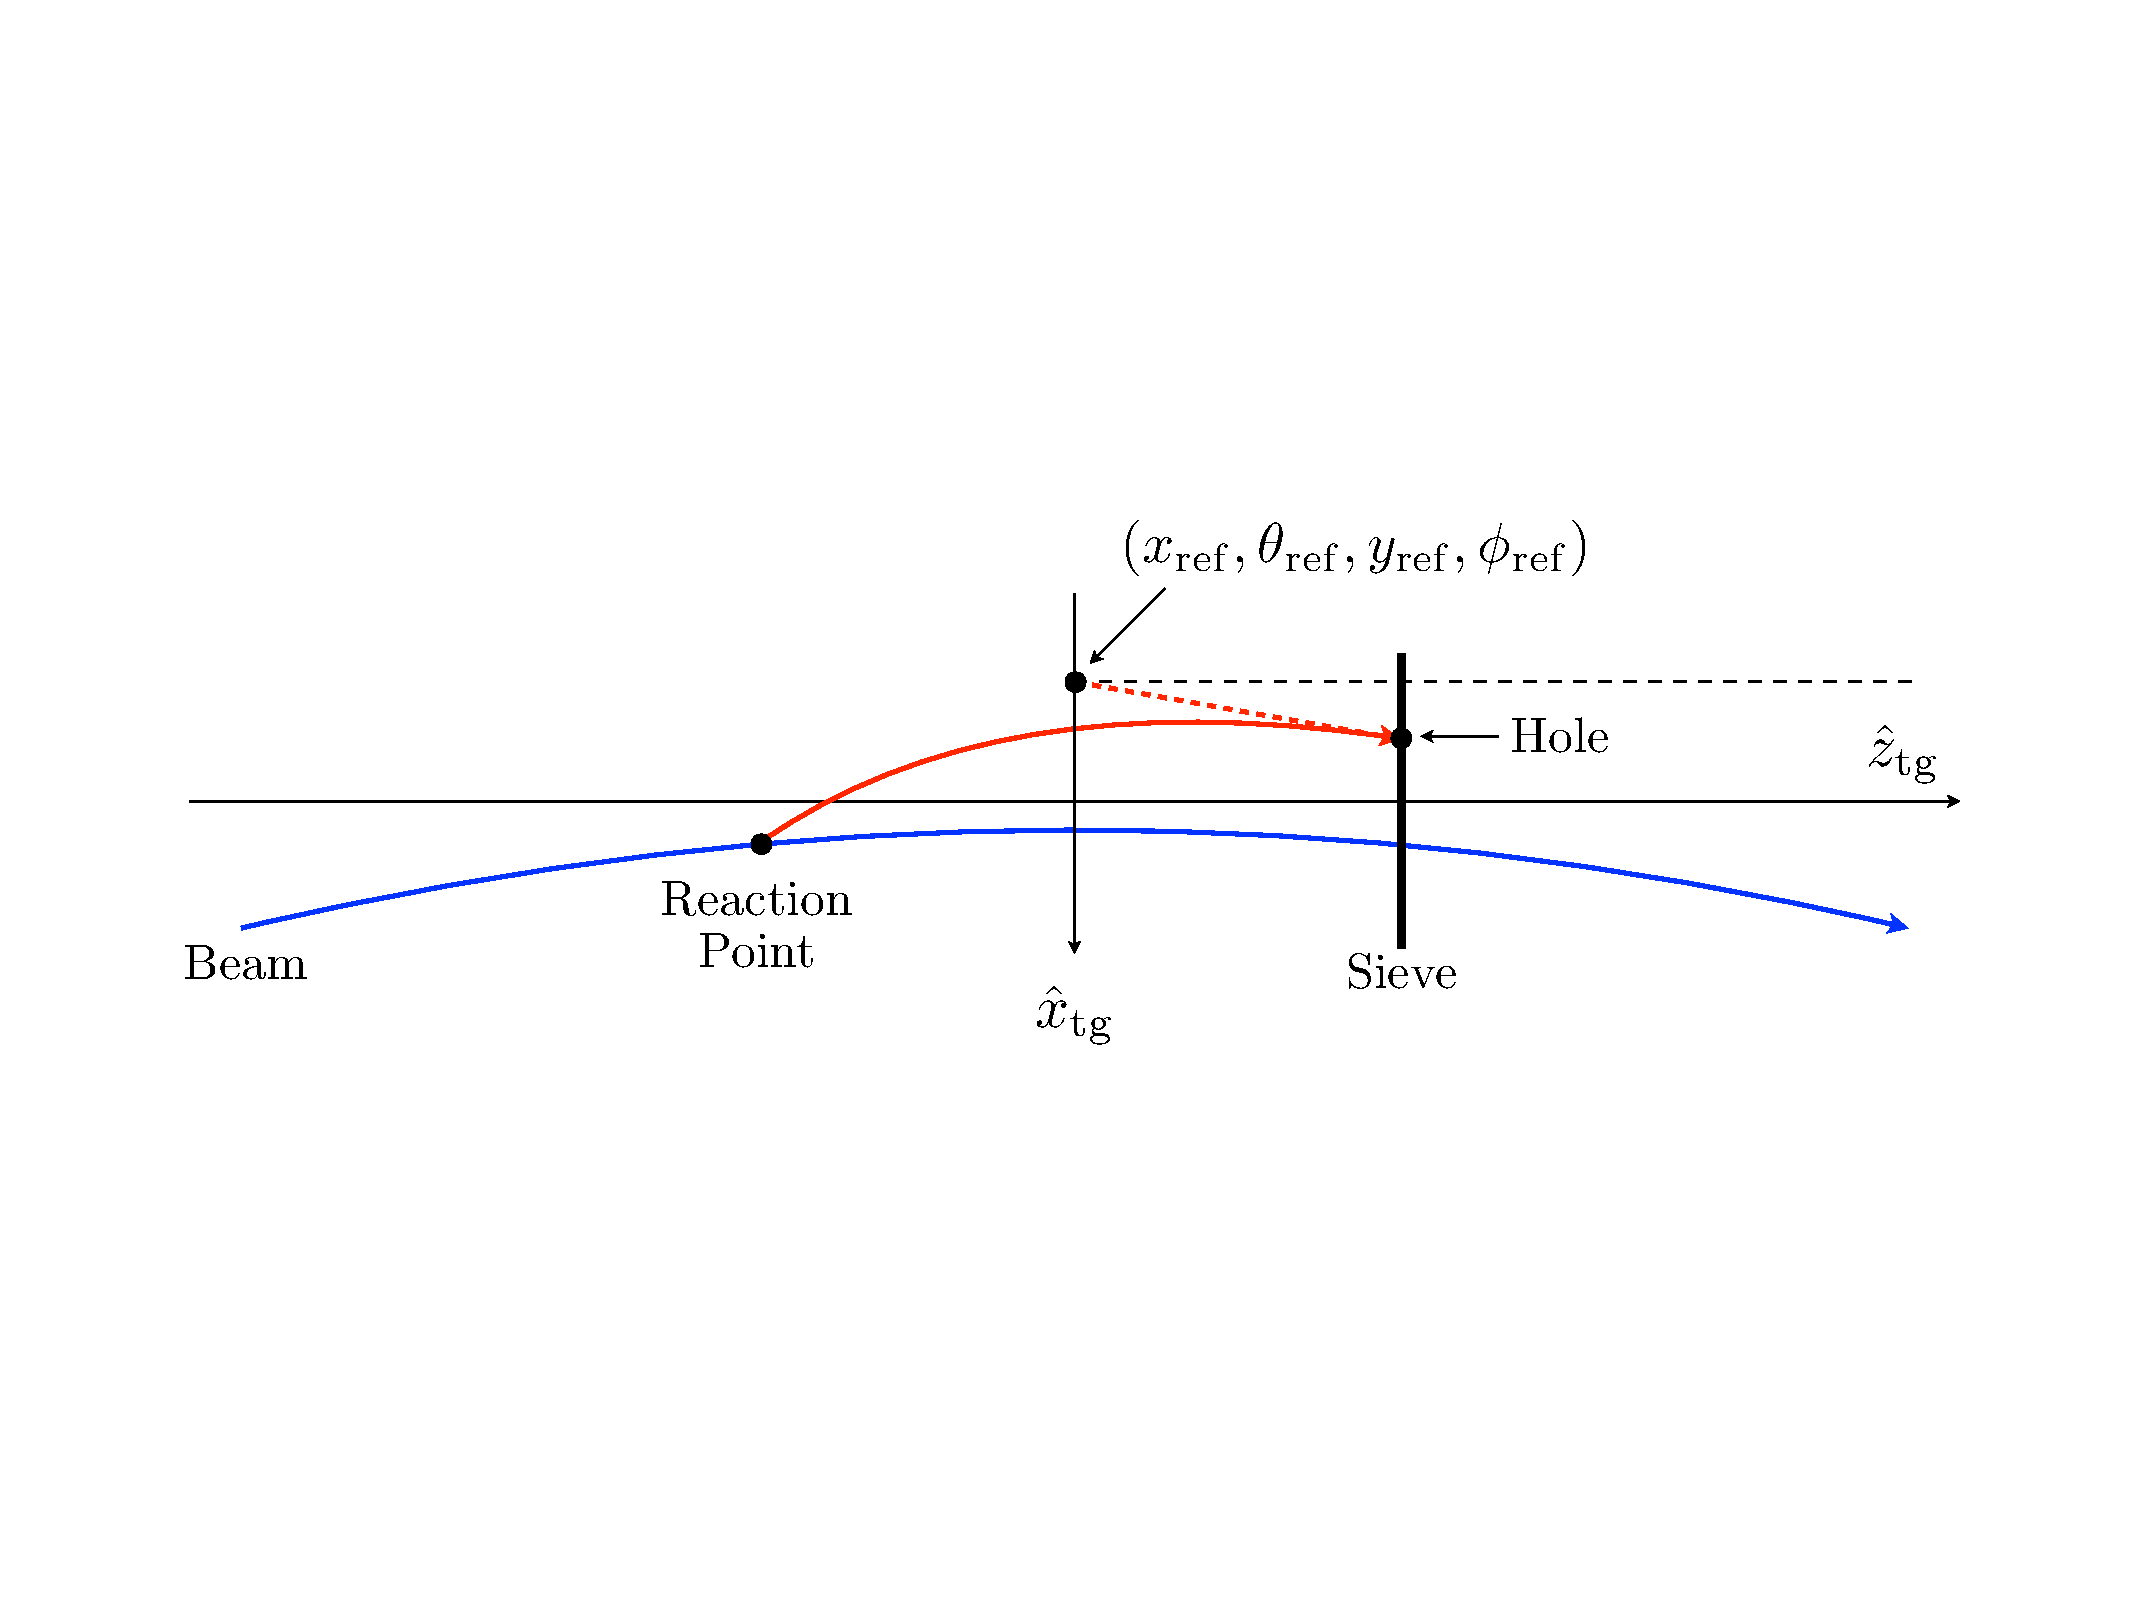
\includegraphics[width=0.9\textwidth]{figs/optics-reference-value.pdf}
  \caption[Determine the new reference values for the optics optimization.]{Determine the new reference values for the optics optimization with simulation. The red trajectory is determined in step \ref{C6S2SS4A1} and \ref{C6S2SS4A2}. \label{C6S2SS4F1}}
\end{figure}

\item Repeat step \ref{C6S2SS4A1} and \ref{C6S2SS4A2} until the deviation between the simulated point ($\optx{drift}$, $\opty{drift}$) and the actual sieve hole position ($\optx{sieve}$, $\opty{sieve}$) is less than the preset tolerance;
\item The trajectory obtained in the final step passes the interaction point and the same sieve hole as the electron passes, step \ref{C6S2SS4A1} assures it simulates an elastic electron. Thus it is the ideal trajectory for this particular event. If the coordinates of this trajectory at its intersection point with the sieve slit is defined as ($\optx{drift}$, $\optt{drift}$, $\opty{drift}$, $\optp{drift}$), the new reference values for the optimization can be obtained by projecting them to the target plane linearly, see \Cref{C6S2SS4F1}:
\begin{align} \label{C6S2SS4E3}
\optx{ref} & = \optx{drift}-L\optt{drift}, & \optt{ref} & = \optt{drift}, \\ \label{C6S2SS4E4}
\opty{ref} & = \opty{drift}-L\optp{drift}, & \optp{ref} & = \optp{drift}.
\end{align}
\end{enumerate}

Once the new reference values are determined, the same algorithm in \cref{C6S2SS2} can be used to do the optimization. A set of Python scripts is added into the original optimization package to calculate the reference values from the survey results with the simulation package. The optimization package is also updated to replace the linear-projected reference values with the new values from the simulation.

\section{Experimental Technique and Results}
\label{C6S3}

\subsection{Required Data}
\label{C6S3SS1}

\Cref{C5T1} summarizes the beam energy and the target field configuration for all kinematic settings. Unfortunately, the septum magnet coils for the right arm of the HRS burned twice during the experiment. Some turns of the coils in the septum were bypassed to fix it, which led to three different septum configurations. They are labeled by the number of the coil turns: ``48-48-16'' for the original septum, ``40-32-16'' for the septum burned once and ``40-00-16'' for the worst case. The septum configuration for each kinematic setting is listed in the septum column of \cref{C5T1}.

The polarized NH${}_3$ target need to be cooled down to 1K in a liquid He (LHe) bath. The LHe container is a cylinder and the diameter is only 42.0 mm. The length of the target is limited by the LHe container to only 28.3 mm along $z$ axis in the HCS. As mentioned in \cref{C6S2SS2}, a set of foil targets is generally used to cover the $\opty{tg}$ acceptance. But at \SI{5.77}{\degree}, the typical position resolution of $\opty{tg}$, $\approx$ 1 mm \cite{Alcorn2004}, is magnified by a factor of 10 in the position along the beam line ($z$ axis in the HCS), which means that the multiple foils installed in the 28.3 mm target cell can not be easily distinguished by the spectrometer. Thus, only one carbon foil is used to collect optics data and we can only optimize $\delta$, $\optt{tg}$ and $\optp{tg}$. The BPM readout is used to determine $y_{tg}$ instead without optics calibration. The thickness of the carbon foil was 40 mil (1.016 mm) for settings 1-5 in \cref{C5T1} and 125 mil (3.175 mm) for the other settings. The foil locations along the beam direction ($\optz{react}$ in \cref{C6S2SS2E1,C6S2SS2E2}) was -13.6 mm for settings 1-5 in \cref{C5T1} and -12.5 mm for the other settings. To reduce the radiation effect, the LHe in the LHe container was vapored and pumped out when collecting the optics data.

The sieve slit used to take optics data is shown in \Cref{C6S2SS2F1}. There are 49 holes in a 7$\times$7 grid pattern with two holes larger than the others. The large holes are used to determine the orientation of the image of the sieve slit. The horizontal distance between the four columns closest to the beam is larger than the distance between the other three columns. This can also be used to determine the orientation in the image. The survey information of the sieve slit was used to calculate the offsets of the central hole from its ideal positions. The $\optx{sieve}$ and $\opty{sieve}$ for each sieve hole is calculated from these offsets and the relative position to the center of the sieve slit. As calculated from the survey result \cite{SurveyA1453,SurveyA1465}, the horizontal offset $D_y$ is 0.0 mm and the vertical offset $D_x$ is -0.2 mm.

The beam position $\optx{beam}$ and $\opty{beam}$ is determined by BPMs. The details of the calibration of the BPMs can be found in reference \cite{Zhu2016}. Because of the target field, the beam is not a straight line in this experiment. The incident angle of the beam at the target can be obtained from the BPM readouts, which can be expressed as the polar angle $\optt{beam}$ and the azimuthal angle $\optp{beam}$ in the HCS. The scattering angle is the angle between the incident beam and the trajectory of the scattered electron, which can be calculated via two auxiliary vectors. The vector describing the beam direction is:
\begin{equation} \label{C6S3SS1E1}
\vec{A} = (\sin(\optt{beam})\cos(\optp{beam}),\ \sin(\optt{beam})\sin(\optp{beam}),\ \cos(\optt{beam})),
\end{equation}
while the vector corresponding to the scattered electron is:
\begin{equation} \label{C6S3SS1E2}
\vec{B} = (\optp{tg}\cos(\theta_0)+\sin(\theta_0),\ -\optt{tg},\ \cos(\theta_0)-\optp{tg}\sin(\theta_0)),
\end{equation}
and the scattering angle is determined as:
\begin{equation} \label{C6S3SS1E3}
\cos\optt{scat} = \frac{\vec{A}\cdot\vec{B}}{|\vec{A}||\vec{B}|},
\end{equation}
where $\optt{beam}$ and $\optp{beam}$ are the azimuthal angles of the incident angle of the beam and $\optt{tg}$ and $\optp{tg}$ are the tangents of the corresponding angles to keep consistent with the definition in the TCS. \cref{C6S3SS1E1,C6S3SS1E2,C6S3SS1E3} replace \cref{C6S1SS2E2} when the beam has an incident angle.

Delta scan was performed by setting $P_0$ at $\pm 3\%$, $\pm 2\%$, $\pm 1\%$ and $0\%$ of the elastic momentum for each configuration except for the one with 3.350 GeV beam energy. In this paticular setting, the elastic scattered electrons can not pass through the septum magnet even if the septum current is set to its upper limit. Since only one foil of carbon target is used in the experiment, the $\opty{tg}$ coverage of the optics calibration was limited. Thus, the incident beam position was adjusted manually by a few millimeters to perform a beam position scan to increase the $\opty{tg}$ coverage. Assuming that the original beam position is (0,0), beam position scan is performed at (0,$\ \pm 4$ mm) and ($\pm 4$ mm,0).

\subsection{Optimization Results}
\label{C6S3SS2}

The optics matrix was optimized for each beam energy and target field configurations listed in \cref{C5T1} except for 3.350 GeV. The procedure discussed in \cref{C6S2SS4} was followed. In this section, the event selection and optimization results are discussed. The data collected with the 1.710 GeV beam energy and 2.5 T transverse target field is taken as an example.

The spectrometer central angle needs to be determined before the matrix calibration. As mentioned in \Cref{C6S2SS2}, the pointing measurement is considered to be more accurate than a survey for the spectrometer central angle determination, since most of the systematic uncertainty can cancel out when considering the difference of the elastic peak. However, in this experiment, although the carbon and the LHe can be used to perform a pointing measurement, the systematic error can not cancel completely due to the fact that the center of the liquid helium region could not be determined accurately. Thus, the survey method was chosen to determine the spectrometer central angle. The result is summarized in \cref{C6S3SS2T1}. More details about the central angle calibration can be found in Ref. \cite{Huang2014}.

\begin{table}[tb!]
  \centering
  \newcolumntype{C}[1]{>{\centering\arraybackslash}m{#1}}
  \begin{tabular}{|c|C{2.5cm}|C{2cm}|}
    \hline
    Arm & Central Angle (rad) \\ \hline
    HRS-L & 0.1007$\pm$0.0007 \\ \hline
    HRS-R & 0.1009$\pm$0.0007 \\ \hline
  \end{tabular}
  \caption[Spectrometer central angles.]{Spectrometer central angles. \label{C6S3SS2T1}}
\end{table}

\begin{figure}[b!]
  \centering
  \begin{subfigure}[t]{0.49\textwidth}
    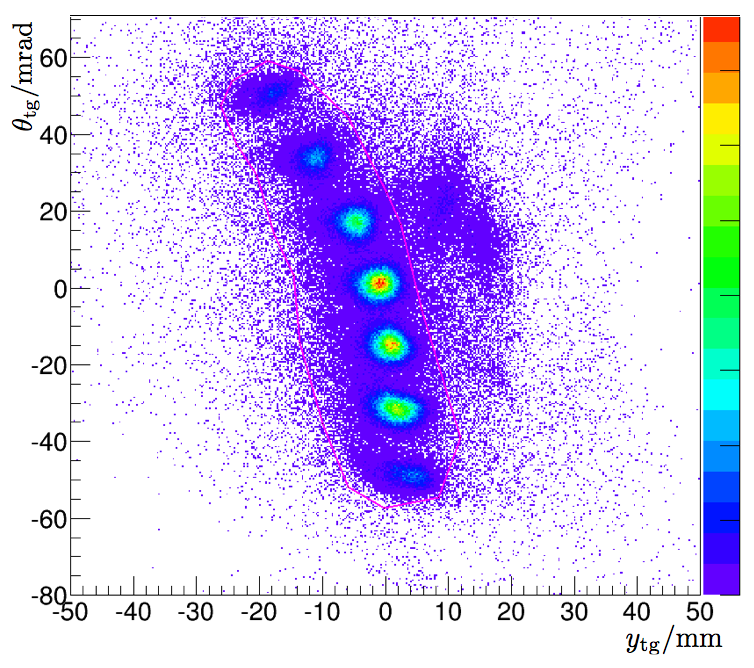
\includegraphics[width=\textwidth]{figs/foil-cut.png}
  \end{subfigure}
  \begin{subfigure}[t]{0.49\textwidth}
    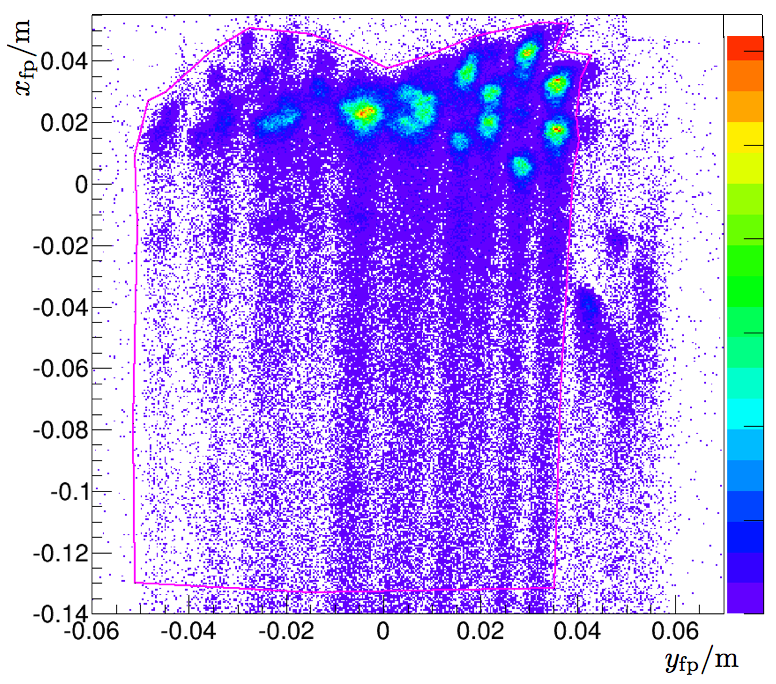
\includegraphics[width=\textwidth]{figs/focal-plane-cut.png}
  \end{subfigure}
  \caption[The foil cut and the focal plane cut.]{The foil cut (left) and the focal plane cut (right). \label{C6S3SS2F1}}
\end{figure}

Before the optics study, the initial matrix generated by SNAKE as mentioned in \cref{C6S2SS2} was used to reconstruct the target variables of the optics data. These target variables were used to make cuts. The data need to be selected by applying several different kinds of cut. Although the carbon foil data is relatively clean, it can still be diluted by electrons scattered from the windows on the target chamber. These events can be removed by applying a foil cut on $\opty{tg}$ or a cut on the focal plane variable $\opty{fp}$ since only one foil was used. The focal plane cut and $\opty{tg}$ cut are shown in \Cref{C6S3SS2F1}, which were chosen empirically. After the foil cut was made, a set of cuts on target variable $\optt{tg}$ and $\optp{tg}$ was made for each hole in the sieve slit. And for each sieve hole, a cut on relative momentum $\delta$ was made to select the elastic events. Since $\opty{tg}$ acceptance is covered by the beam position scan instead of using multiple foils of target, a beam position cut on $\optx{beam}$ and $\opty{beam}$ was also performed to select data with the proper beam position. The cut definition process was repeated for each delta scan and beam position scan configurations. Each cut was assigned with an identification number and saved to a separate file.

The optimization package uses the saved cuts to select events. The FCS coordinates, positions and angles of the beam and the identification number of the cut for selected events are recorded into a ASCII file. The script mentioned in \Cref{C6S2SS4} uses the file as an input to calculate the reference values for optimization, and append the reference values to the focal plane variables for each event in the file. For example, the reference values of $\optt{tg}$ and $\optp{tg}$ for 1.710 GeV configuration is shown in the left panel of \Cref{C6S3SS2F2}. The focal plane variables and the reference values are read by the updated optimization program from the file to optimize the optics matrix.

\begin{figure}[tb!]
  \centering
  \begin{subfigure}[t]{0.45\textwidth}
    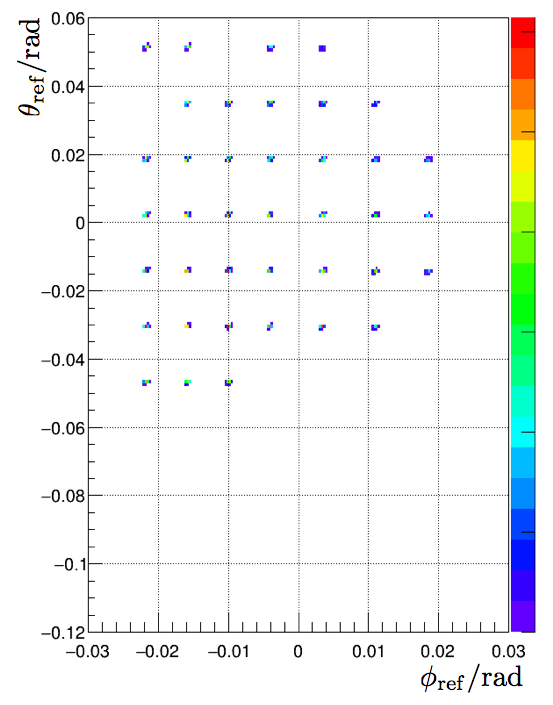
\includegraphics[width=\textwidth]{figs/reference-angle-simulation.png}
  \end{subfigure}
  \begin{subfigure}[t]{0.45\textwidth}
    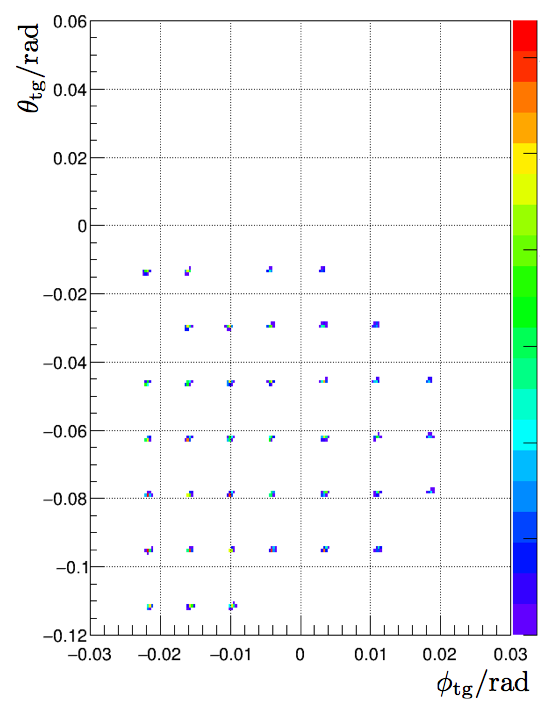
\includegraphics[width=\textwidth]{figs/initial-angle-simulation.png}
  \end{subfigure}
  \caption[Reference values for angular optimization.]{The reference values of $\optt{tg}$ and $\optp{tg}$ for optimization (left) and the corresponding actual target plane angle at the reaction point (right). The difference between the two panels is due to the target field, which was determined from the simulation described in \Cref{C6S2SS3}. \label{C6S3SS2F2}}
\end{figure}

\begin{figure}[b!]
  \centering
  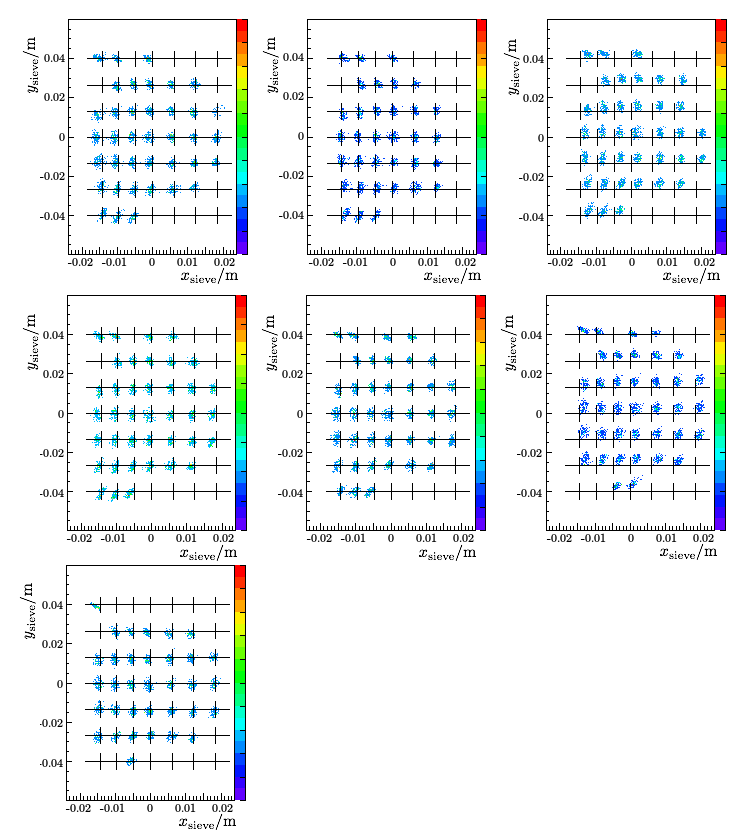
\includegraphics[width=\textwidth]{figs/sieve-pattern.png}
  \caption[Sieve Pattern for 1.710 GeV data.]{Sieve Pattern for 1.710 GeV data. The patterns of different delta scans are shown in separate plots. The three plots in the top row is delta scans with spectrometer central momenta ($P_0$) setting to $+3\%$ (left), $+2\%$ (center) and $0\%$ (right) of the elastic momentum, the bottom row is delta scans with $P_0$ setting to $-2\%$ (left) and $-3\%$ (center). The cross points of the grids in the plots are used to indicate the actual positions of the sieve holes. The good agreement between the hole images and the grid indicates the angles $\optt{tg}$ and $\optp{tg}$ have been calibrated well. \label{C6S3SS2F3}}
\end{figure}

The angular components of the optics matrix are optimized first. The optimized matrix is used to reconstruct the target variables. The sieve pattern is generated by the projection of the reconstructed $\optt{tg}$ and $\optp{tg}$ from the interaction point to the sieve slit plane. The sieve pattern for the 1.710 GeV data is shown in \Cref{C6S3SS2F3}. The nominal position of the sieve holes are indicated by the cross points of the grids in the plots.

\begin{figure}[tb!]
  \centering
  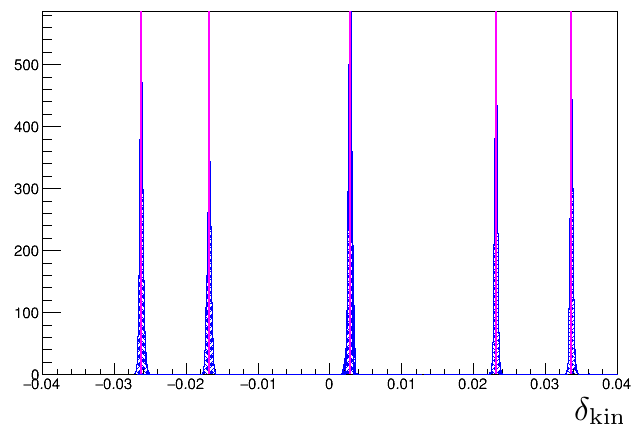
\includegraphics[width=0.6\textwidth]{figs/delta-pattern.png}
  \caption[The $\delta_{\mathrm{kin}}$ calibration results for 1.710 GeV data.]{The $\delta_{\mathrm{kin}}$ calibration results for 1.710 GeV data. The peaks in the plot are the reconstructed $\delta_{\mathrm{kin}}$ from different delta scan configurations, summed over all sieve holes. Starting from the left, the spectrometer central momenta are $+3\%$, $+2\%$, $0\%$, $-2\%$ and $-3\%$ of the elastic momentum respectively. The magenta lines in the plots indicate the actual value of the $\delta_{\mathrm{kin}}$. \label{C6S3SS2F4}}
\end{figure}

Next step is the momentum calibration. As shown in \cref{C6S2SS2}, the momentum of an elastically scattered electron depends on the scattering angle. Since the sieve slit covers a wide angle range, the scattering angles of the electrons passing through different sieve holes are different. The elastic peak is broadened due to this effect, which influences the resolution of the optimization. Thus, a new variable is defined to remove the angular dependence of $\delta$:
\begin{equation} \label{C6S3SS2E1}
\delta_{\mathrm{kin}} = \delta - \frac{P(M,\ \theta)-P(M,\, \theta_0)}{P_0},
\end{equation}
where $\theta_0$ is the spectrometer central angle and $\theta$ is the scattering angle. The second term on the right hand side of \cref{C6S3SS2E1} is defined as $\delta_{\mathrm{corr}}$:
\begin{equation} \label{C6S3SS2E2}
\delta = \delta_{\mathrm{kin}} + \delta_{\mathrm{corr}}(M, \theta).
\end{equation}
$\delta_{\mathrm{corr}}$ only depends on the target material and the scattering angle. In practice, $\delta_{\mathrm{corr}}$ is calculated with the survey result and the beam positions before the optimization starts. During the optimization, the saved $\delta_{\mathrm{corr}}$ can be used to convert $\delta$ to $\delta_{\mathrm{kin}}$ with almost no additional computing cost. Momentum $\delta_{\mathrm{kin}}$ for events from different sieve holes can then be optimized together. The $\delta_{\mathrm{kin}}$ calibration results for 1.710 GeV data are shown in \Cref{C6S3SS2F4}. The nominal positions of the $\delta_{\mathrm{kin}}$ are indicated by magenta lines for each delta scan configuration.

\begin{table}[tb!]
  \centering
  \newcolumntype{C}[1]{>{\centering\arraybackslash}m{#1}}
  \begin{tabular}{|c|C{2.2cm}|C{2.2cm}|}
    \hline
     & Left Arm & Right Arm \\ \hline
    $\delta_{\mathrm{res}}$ & 1.5$\times10^{-4}$ & 2.4$\times10^{-4}$ \\ \hline
    $\theta_{\mathrm{res}}$ (mrad) & 1.6 & 1.6 \\ \hline
    $\phi_{\mathrm{res}}$ (mrad) & 1.0 & 0.8 \\ \hline
  \end{tabular}
  \caption[Summary of the optics performance without target field.]{Summary of the optics performance without target field. $\delta_{\mathrm{res}}$, $\theta_{\mathrm{res}}$ and $\phi_{\mathrm{res}}$ are resolutions in $\delta$, $\theta$ and $\phi$, respectively. \label{C6S3SS2T2}}
\end{table}

\begin{table}[tb!]
  \centering
  \newcolumntype{C}[1]{>{\centering\arraybackslash}m{#1}}
  \begin{tabular}{|c|C{1.7cm}|C{1.7cm}|C{1.2cm}|c|c|C{1.2cm}|C{1.2cm}|}
    \hline
    HRS & Beam Energy (GeV) & Field Strength (T) & Field Angle & Septum & $\delta_{\mathrm{res}}$ & $\theta_{\mathrm{res}}$ (mrad) & $\phi_{\mathrm{res}}$ (mrad) \\ \hline
    L & 2.254 & 2.5 & \SI{90}{\degree} & 48-48-16 & 2.0$\times10^{-4}$ & 1.7 & 1.7 \\ \hline
    L & 2.254 & 2.5 & \SI{90}{\degree} & 40-32-16 & 2.2$\times10^{-4}$ & 1.8 & 1.8 \\ \hline
    L & 1.710 & 2.5 & \SI{90}{\degree} & 40-00-16 & 2.4$\times10^{-4}$ & 2.4 & 1.5 \\ \hline
    L & 1.157 & 2.5 & \SI{90}{\degree} & 40-00-16 & 3.2$\times10^{-4}$ & 2.1 & 1.3 \\ \hline
    L & 2.254 & 5.0 & \SI{0}{\degree} & 40-00-16 & 2.2$\times10^{-4}$ & 1.6 & 1.2 \\ \hline
    R & 2.254 & 2.5 & \SI{90}{\degree} & 48-48-16 & 1.8$\times10^{-4}$ & 1.6 & 1.2 \\ \hline
    R & 2.254 & 2.5 & \SI{90}{\degree} & 40-32-16 & 2.5$\times10^{-4}$ & 2.2 & 1.8 \\ \hline
    R & 1.710 & 2.5 & \SI{90}{\degree} & 40-00-16 & 2.3$\times10^{-4}$ & 2.7 & 1.7 \\ \hline
    R & 1.157 & 2.5 & \SI{90}{\degree} & 40-00-16 & 3.4$\times10^{-4}$ & 1.9 & 1.5 \\ \hline
  \end{tabular}
  \caption[Summary of optics performance with the target field.]{Summary of optics performance with the target field. Here ``L'' and ``R'' stand for the left arm and right arm of the HRS. $\delta_{\mathrm{res}}$, $\theta_{\mathrm{res}}$ and $\phi_{\mathrm{res}}$ are resolutions in $\delta$, $\theta$ and $\phi$, respectively. \label{C6S3SS2T3}}
\end{table}

In this section, only the optimization results for 1.710 GeV configuration is shown as an example. However the optimization was performed for all kinematic settings and the optics data without target field was optimized as well with the normal procedure to verify the HRS performance. The resolutions of the optics matrix without the target field is summarized in \cref{C6S3SS2T2} and the resolutions of the optics matrix with target field is summarized in \cref{C6S3SS2T3}. Here the resolution is evaluated via:
\begin{equation} \label{C6S3SS2E3}
f_{\mathrm{res}}^W = \sqrt{\frac{1}{N}\sum_{s=1}^N(W_s-W_s^0)^2},
\end{equation}
where $W$ are calculated with optics matrix, $W_0$ are the reference values and $N$ is the total number of the events used in the optimization. See Ref. \cite{OPTICSWIKI} for more plots of the optimization results for each setting listed in \cref{C5T1}.

\section{Reconstruction Procedure}
\label{C6S4}

Since the final purpose of the optics study is to reconstruct the kinematic variables for each event, the reconstruction procedure is included as part of the optics study. If there is no target field, the Hall A Analyzer is designed to read the optics matrix and calculate the target plane variables directly for each event \cite{Hansen2015} and no additional process is required. However, this is not the case with the target field.

\begin{figure}[b!]
  \centering
  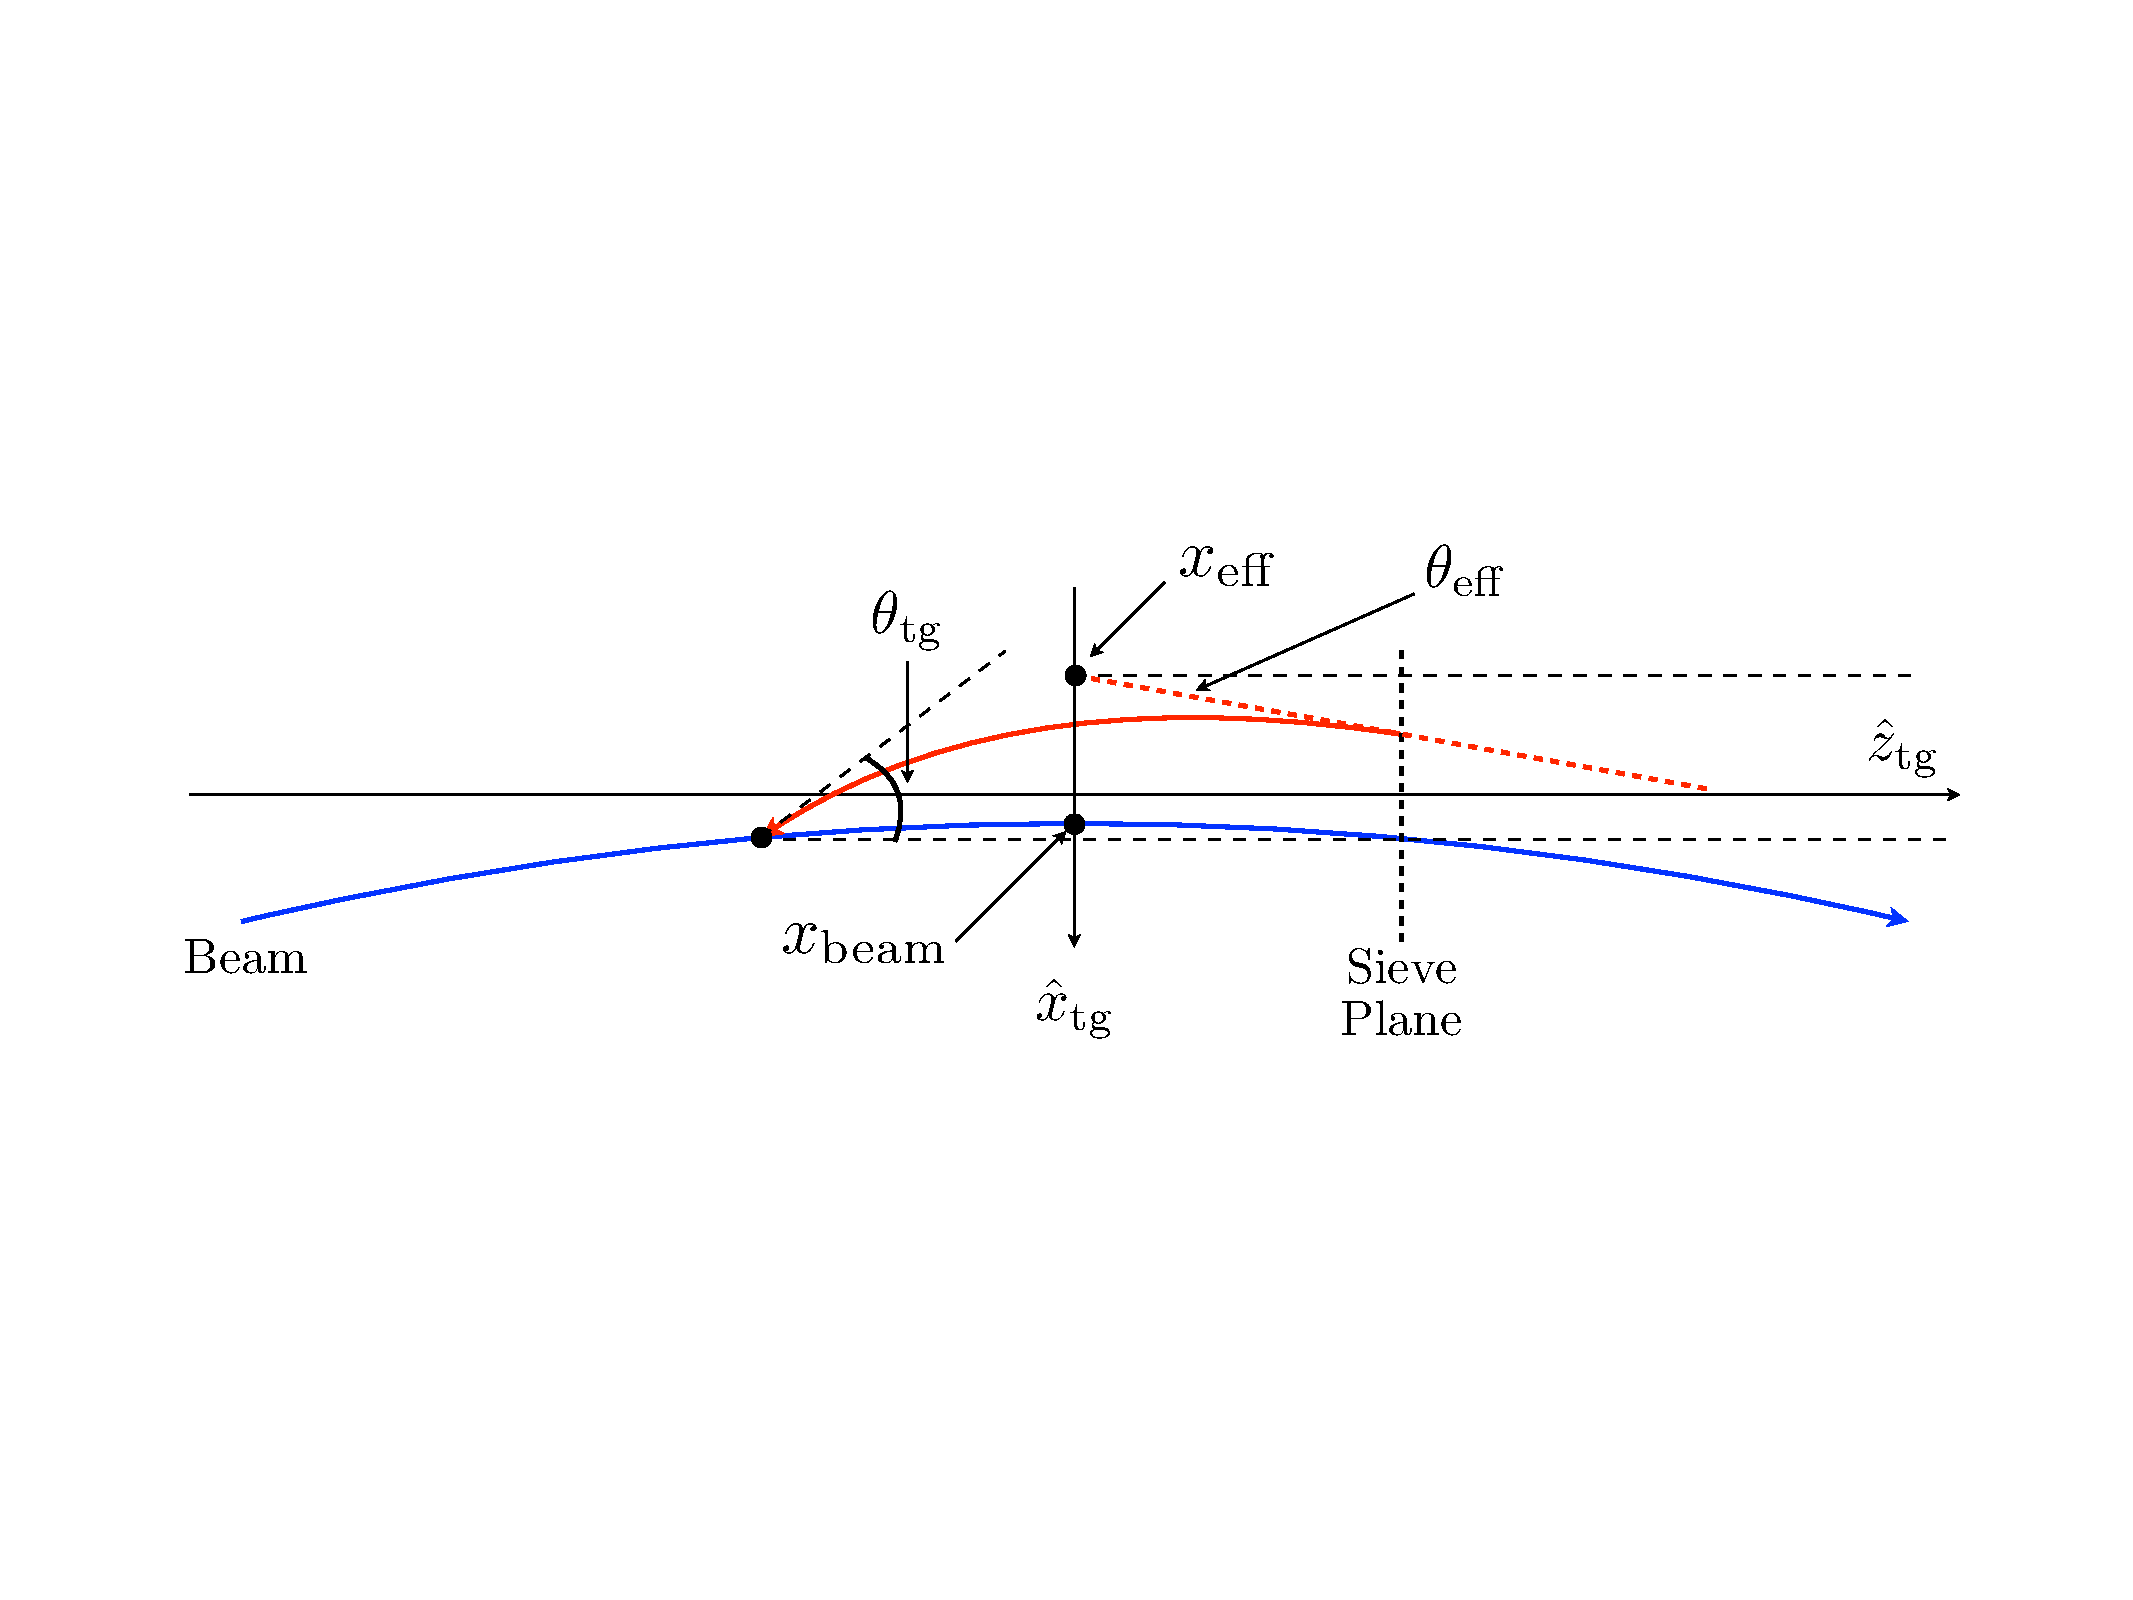
\includegraphics[width=0.9\textwidth]{figs/reconstruction.pdf}
  \caption[Reconstruction of the target kinematic variables.]{Reconstruction of the target kinematic variables. Here $\optt{eff}$ is reconstrcted by the optics matrix from the focal plane variable. The red dot line shows the linear projection to the sieve slit plane and the read solid line indicates the trojectory generated by the simulation package, which gives us the real target variable $\optt{tg}$. The detailed procudure is discussed in this section.  \label{C6S4F1}}
\end{figure}

Following the logic in \Cref{C6S2SS4}, the reconstruction procedure can also be completed in two steps. The first step is to reconstruct the coordinates of the intersection point of the scattered electron and the sieve slit plane, which can be obtained from the focal plane variables with the optimized optics matrix. The second step is to determine the trajectory of the electron from the sieve slit plane to the target with the simulation package. The detailed procedure to reconstruct kinematic variables involve the following steps:
\begin{enumerate}[parsep=0pt]
\item \label{C6S4A1} Select an event, apply the optics matrix to the focal plane coordinates ($\optx{fp}$, $\optt{fp}$, $\opty{fp}$, $\optp{fp}$) to calculate the relative momentum $\delta$ and the effective target angles $\optt{eff}$ and $\optp{eff}$ at the target plane, which is the $z=0$ plane in TCS. In practice, this step is performed by the Hall A Analyzer;
\item \label{C6S4A2} Calculate the effective beam positions $\optx{eff}$ and $\opty{eff}$ in TCS from the actual beam positions provided by BPMs with the target field simulation described later. Combine with the angles obtained in step \ref{C6S4A1}, the effective target variables are ($\optx{eff}$, $\optt{eff}$, $\opty{eff}$, $\optp{eff}$);
\item Perform a linear projection of ($\optx{eff}$, $\optt{eff}$, $\opty{eff}$, $\optp{eff}$) to the sieve slit plane, which is the $z=L$ plane in TCS, to obtain ($\optx{proj}$, $\optt{proj}$, $\opty{proj}$, $\optp{proj}$);
\item Set ($\optx{proj}$, $\opty{proj}$, $\optz{proj}=L$) as the start point and set the $\delta$ and ($\optt{proj}$, $\optp{proj}$) as the magnitude and direction of the momentum respectively, use the simulation package to generate a trajectory from the start point to the target plane in TCS, which gives the target variables ($\optx{tg}$, $\optt{tg}$, $\opty{tg}$, $\optp{tg}$) of the selected event.
\end{enumerate}

\begin{figure}[b!]
  \centering
  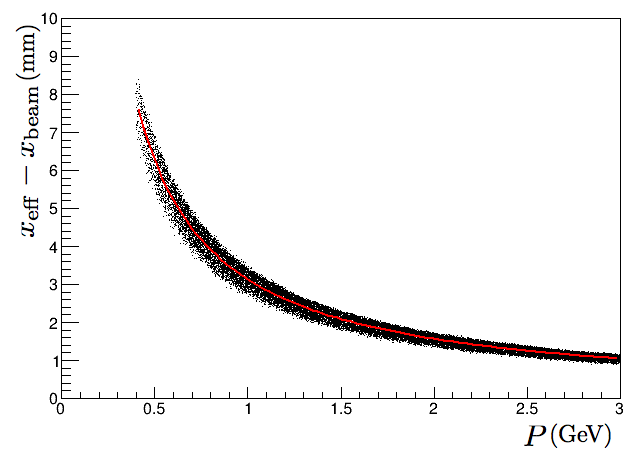
\includegraphics[width=0.6\textwidth]{figs/effective-x-fit.png}
  \caption[Determine the effective beam position correction.]{The relation between $\optx{eff}-\optx{beam}$ and the momentum of the scattered electron from the simulation. The red curve is the fit result of the function in \cref{C6S4E1}. \label{C6S4F2}}
\end{figure}

\begin{table}[b!]
  \centering
  \newcolumntype{C}[1]{>{\centering\arraybackslash}m{#1}}
  \begin{tabular}{|C{1.2cm}|C{2.3cm}|C{1.8cm}|C{2.2cm}|C{1.8cm}|C{2.2cm}|}
    \hline
    HRS & Field & $C_0^{\,x}$ (mm) & $C_1^{\,x}$ (mm$\cdot$GeV/c) & $C_0^{\,y}$ (mm) & $C_1^{\,y}$ (mm$\cdot$GeV/c) \\ \hline
    Left & 2.5 T at \SI{90}{\degree} & 0.00 & 3.14 & -0.09 & 0.22 \\ \hline
    Left & 5.0 T at \SI{0}{\degree} & 0.00 & -0.75 & 0.16 & -0.40 \\ \hline
    Left & 5.0 T at \SI{90}{\degree} & -0.04 & 6.34 & -0.35 & 0.86 \\ \hline
    Right & 2.5 T at \SI{90}{\degree} & 0.00 & 3.13 & 0.09 & -0.21 \\ \hline
    Right & 5.0 T at \SI{0}{\degree} & 0.00 & 0.76 & -0.15 & 0.34 \\ \hline
    Right & 5.0 T at \SI{90}{\degree} & -0.05 & 6.37 & 0.35 & -0.85 \\ \hline
  \end{tabular}
  \caption[Fit parameters of effective beam position correction.]{Fit parameters of the effective beam position correction. \label{C6S4T1}}
\end{table}

The effective beam positions $\optx{eff}$ and $\opty{eff}$ used in step \ref{C6S4A2} is generated by adding a correction to actual position, $\optx{beam}$ and $\opty{beam}$, of the scattered electron. The correction is defined as $\optx{eff}-\optx{beam}$, which is plotted in \Cref{C6S4F2} for 2.5 T transverse target field setting as an example. Since the target in this experiment is short, the $\optx{eff}-\optx{beam}$ term is dominated by the deviation of the linear projection from the actual trajectory. The deviation shows a strong correlation with the momentum $P$ of the scattered electron due to the target field. The simulated $\optx{eff}-\optx{beam}$ values can be fit as a function of $P$:
\begin{equation} \label{C6S4E1}
\optx{eff}-\optx{beam} = C_0 + C_1/P.
\end{equation}
Similar expressions can be written for $\opty{eff}$ and $\opty{beam}$. The fit is performed for all three target field configurations on both spectrometers. The fit parameters are summarized in \cref{C6S4T1}.

A Python script was developed to calculate the kinematic variables following the procedure described above. The original reconstruction script based on the Hall A analyzer is included in this script as a preprocessor of the data.

%%%%%%%%%%%%%%%%%%%%%%%%%%%%%%%%%%%%%%%%%%%%%%%%%%%%%%%%%%%%%%%%%%%%%%
% -*-latex-*-
